% Paquets généraux
\documentclass[a4paper,12pt,titlepage]{article}
\usepackage[T1]{fontenc}
\usepackage[utf8]{inputenc}
\usepackage[french]{babel}
\usepackage[gen]{eurosym}
%\usepackage[dvips]{graphicx}
\usepackage{fancyhdr}
\usepackage{pdfpages} 
\usepackage{multido}
\usepackage{hyperref}
%\usepackage{textcomp}
%\usepackage{aeguill}
\usepackage{schemabloc}
\usepackage[bitstream-charter]{mathdesign}

\newcommand{\id}{54}
\newcommand{\nom}{Liaisons mécaniques}
\newcommand{\sequence}{04}
\newcommand{\num}{01}
\newcommand{\type}{TP}
\newcommand{\descrip}{Modélisation d'un solide. Comportement des liaisons mécaniques. Modéliser les mécanismes du laboratoire par un schéma cinématique, paramétré.}
\newcommand{\competences}{A3-C4: Analyse d'architecture et de comportement \\ &  Mod1-C1: Isolement d'un solide ou d'un système de solides \\ &  Mod2-C10-1: Modèle de solide indéformable \\ &  Mod2-C11: Modélisation géométrique et cinématique des mouvements entre solides indéformables \\ &  Mod2-C12: Modélisation cinématique des liaisons entre solides \\ &  Mod2-C15: Modélisation des actions mécaniques \\ &  Rés-C6: Utilisation d'un solveur ou d'un logiciel multi physique \\ &  Com1-C1: Différents descripteurs introduits dans le programme \\ &  Com2-C4: Outils de communication}
\newcommand{\nbcomp}{9}
\newcommand{\systemes}{Plateforme Stewart}
\newcommand{\systemessansaccent}{Plateforme Stewart}
\newcommand{\ilot}{2}
\newcommand{\ilotstr}{02}
\newcommand{\dossierilot}{\detokenize{Ilot_02 Plateforme Stewart}}
\newcommand{\imageun}{Plateforme}

\newcommand{\urlsysteme}{\href{https://www.costadoat.fr/systeme/57}{Ressources système}}
\newcommand{\matlabsimscape}{\href{https://github.com/Costadoat/Sciences-Ingenieur/raw/master/Systemes/Plateforme Stewart/Plateforme_Stewart_Simscape.zip}{Modèle Simscape}}
\newcommand{\solidworks}{\href{https://github.com/Costadoat/Sciences-Ingenieur/raw/master/Systemes/Plateforme Stewart/Plateforme_Stewart_Solidworks.zip}{Modèle Solidworks}}
\newcommand{\edrawings}{\href{https://github.com/Costadoat/Sciences-Ingenieur/raw/master/Systemes/Plateforme Stewart/Plateforme_Stewart.EASM}{Modèle eDrawings}}
\newcommand{\test}{Stewart_param1}
\newcommand{\testi}{Stewart_param2}
\newcommand{\testii}{Stewart_param3}
\newcommand{\testiii}{Stewart_param4}
\newcommand{\testiiii}{Stewart_euler}

\newcommand{\auteurun}{Renaud Costadoat}
\newcommand{\auteurdeux}{Françoise Puig}
\newcommand{\institute}{Lycée Dorian}


\usepackage{color}
\usepackage{xcolor}
\usepackage{colortbl}
\usepackage{helvet}
\renewcommand{\familydefault}{\sfdefault}
\usepackage{amsfonts}
\usepackage{amsmath}
%\usepackage{xspace}
\usepackage{varioref}
\usepackage{tabularx}
%\usepackage{floatflt}
\usepackage{graphics}
\usepackage{wrapfig}
\usepackage{textcomp}
\usepackage{tikz}
\usepackage{wrapfig}
\usepackage{gensymb}
\usepackage[european]{circuitikz}
\usetikzlibrary{babel}
\usepackage{ifthen}
\usepackage{cancel}
\usepackage{etoolbox}
\usepackage{multirow}
%\usepackage{boxedminipage}
\definecolor{gris25}{gray}{0.75}
\definecolor{bleu}{RGB}{18,33,98}
\definecolor{bleuf}{RGB}{42,94,171}
\definecolor{bleuc}{RGB}{231,239,247}
\definecolor{rougef}{RGB}{185,18,27}
\definecolor{rougec}{RGB}{255,188,204}%255,230,231
\definecolor{vertf}{RGB}{103,126,82}
\definecolor{vertc}{RGB}{220,255,191}
\definecolor{forestgreen}{rgb}{0.13,0.54,0.13}
\definecolor{blcr}{rgb}{0.59,0.69,0.84}
\definecolor{blfr}{rgb}{0.32,0.51,0.75}
\definecolor{orfr}{rgb}{0.90,0.42,0.15}
\definecolor{orcr}{rgb}{0.90,0.65,0.50}
\definecolor{orangef}{rgb}{0.659,0.269,0.072}
\definecolor{orange}{rgb}{0.58,0.35,0.063}
\definecolor{orangec}{rgb}{0.43,0.32,0.25}
\definecolor{rcorrect}{rgb}{0.6,0,0}
\definecolor{sequence}{rgb}{0.75,0.75,0.75}
\definecolor{competences}{rgb}{0.61,0.73,0.35}
\definecolor{grisf}{HTML}{222222}
\definecolor{grisc}{HTML}{636363}
\definecolor{normal}{HTML}{4087c4}
\definecolor{info}{HTML}{5bc0de}
\definecolor{success}{RGB}{92,184,92}
\definecolor{warning}{RGB}{240,173,78}
\definecolor{danger}{RGB}{217,83,79}
\hypersetup{                    % parametrage des hyperliens
    colorlinks=true,                % colorise les liens
    breaklinks=true,                % permet les retours à la ligne pour les liens trop longs
    urlcolor= blfr,                 % couleur des hyperliens
    linkcolor= orange,                % couleur des liens internes aux documents (index, figures, tableaux, equations,...)
    citecolor= forestgreen                % couleur des liens vers les references bibliographiques
    }

% Mise en page
\pagestyle{fancy}

\setlength{\hoffset}{-18pt}

\setlength{\oddsidemargin}{0pt} 	% Marge gauche sur pages impaires
\setlength{\evensidemargin}{0pt} 	% Marge gauche sur pages paires
\setlength{\marginparwidth}{00pt} 	% Largeur de note dans la marge
\setlength{\headwidth}{481pt} 	 	% Largeur de la zone de tête (17cm)
\setlength{\textwidth}{481pt} 	 	% Largeur de la zone de texte (17cm)
\setlength{\voffset}{-18pt} 		% Bon pour DOS
\setlength{\marginparsep}{7pt}	 	% Séparation de la marge
\setlength{\topmargin}{-30pt} 		% Pas de marge en haut
\setlength{\headheight}{35pt} 		% Haut de page
\setlength{\headsep}{20pt} 		% Entre le haut de page et le texte
\setlength{\footskip}{30pt} 		% Bas de page + séparation
\setlength{\textheight}{700pt} 		% Hauteur de l'icone zone de texte (25cm)
\setlength\fboxrule{1 pt}
\renewcommand{\baselinestretch}{1}
\setcounter{tocdepth}{1}
\newcommand{\cadre}[2]
{\fbox{
  \begin{minipage}{#1\linewidth}
   \begin{center}
    #2\\
   \end{center}
  \end{minipage}
 }
}

\newcounter{num_quest} \setcounter{num_quest}{0}
\newcounter{num_rep} \setcounter{num_rep}{0}
\newcounter{num_cor} \setcounter{num_cor}{0}

\newcommand{\question}[1]{\refstepcounter{num_quest}\par
~\ \\ \parbox[t][][t]{0.15\linewidth}{\textbf{Question \arabic{num_quest}}}\parbox[t][][t]{0.93\linewidth}{#1}\par
}


\newcommand{\reponse}[1]
{\refstepcounter{num_rep}
\noindent
\rule{\linewidth}{.5pt}
\textbf{Question \arabic{num_rep}:}
\multido{\i=1+1}{#1}{~\ \\}
}

\newcommand{\cor}
{\refstepcounter{num_cor}
\noindent
\rule{\linewidth}{.5pt}
\textbf{Question \arabic{num_cor}:} \\
}

\newcommand{\titre}[1]
{\begin{center}
\cadre{0.8}{\huge #1} 
\end{center}
}


% En tête et pied de page
\fancypagestyle{normal}{%
  \fancyhf{}
\lhead{\nom}
\rhead{
\includegraphics[width=2cm]{../../img/logo}\hspace{2pt}}
\ifdef{\auteurdeux}{\lfoot{\auteurun,\auteurdeux}}{\lfoot{\auteurun}}
\cfoot{Page \thepage}}

\fancypagestyle{correction}{%
  \fancyhf{}
  \lhead{\colorbox{danger}{\begin{minipage}{0.65\paperwidth} \textcolor{white}{\textbf{Correction}} \end{minipage}} }
  \rhead{
\includegraphics[width=2cm]{../../img/logo}}
  \ifdef{\auteurdeux}{\lfoot{\auteurun,\auteurdeux}}{\lfoot{\auteurun}}
  \rfoot{\colorbox{danger}{\begin{minipage}{0.5\paperwidth} \begin{flushright}\textcolor{white}{\textbf{Correction}}\end{flushright} \end{minipage}} }}

\renewcommand{\footrulewidth}{0.4pt}

\usepackage{eso-pic}
\newcommand{\BackgroundPic}{%
\put(0,0){%
\parbox[b][\paperheight]{\paperwidth}{%
\vfill
\begin{center}
\hspace{0.5cm}\vspace{0.5cm}

\includegraphics[width=\paperwidth,height=\paperheight,%
keepaspectratio]{../../img/fond3}%
\end{center}
\vfill
}}}

\newcommand{\BackgroundPicdeux}{%
\put(25,-30){%
\parbox[b][\paperheight]{\paperwidth}{%
\vfill
\begin{center}

\includegraphics[width=\paperwidth,height=\paperheight,%
keepaspectratio]{../../img/fond4}%
\end{center}
\vfill
}}}

\begin{document}

\pagestyle{empty}

\vspace*{-3\baselineskip}

\AddToShipoutPicture*{\BackgroundPic}

\ifdef{\auteurdeux}{\begin{tabular}{>{\columncolor{gray!00}}m{.3\linewidth} m{.3\linewidth} >{\columncolor{gray!00}}m{.3\linewidth}}
Séquence : \sequence &  \multirow{3}{*}{\hspace{1cm}
\includegraphics[height=1.5cm]{../../img/logo}} &  \begin{flushright} \multirow{4}{*}{\hspace{1cm}
\includegraphics[height=4cm]{img/qrcode}}\end{flushright}\\
Document : \type\num \\
 \institute \\
 \auteurun\\
 \auteurdeux
\end{tabular}}{\begin{tabular}{>{\columncolor{gray!00}}m{.3\linewidth} m{.3\linewidth} >{\columncolor{gray!00}}m{.3\linewidth}}
Séquence : \sequence &  \multirow{3}{*}{\hspace{1cm}
\includegraphics[height=1.5cm]{../../img/logo}} &  \begin{flushright} \multirow{4}{*}{\hspace{1cm}
\includegraphics[height=4cm]{img/qrcode}}\end{flushright}\\
Document : \type\num \\
 \institute \\
 \auteurun
\end{tabular}}

\vspace{1cm}

\ifdef{\prive}{\begin{center}\colorbox{danger}{\Huge{Avec Correction}}\end{center}}{}

\begin{center}\huge{\nom}\end{center}

\vspace{2cm}

\ifdef{\imagedeux}{\begin{minipage}{0.49\linewidth}}{}
\begin{center}\includegraphics[height=5cm]{/home/renaud/Documents/Renaud/GitHub/django_education/systemes/\imageun}\end{center}
\ifdef{\imagedeux}{\end{minipage}\hfill
\begin{minipage}{0.49\linewidth}
\begin{center}\includegraphics[height=5cm]{/home/renaud/Documents/Renaud/GitHub/django_education/systemes/\imagedeux}\end{center}
\end{minipage}}{}

\vspace{5cm}


\begin{tabular}{p{.15\linewidth} >{\columncolor{white}}p{.8\linewidth}}
    \rowcolor{gray!20}
    Référence & S\sequence\ - \type\num \\
    Compétences & \competences \\
 	\rowcolor{gray!20}
    Description & \descrip \\
    Système & \systemes
  \end{tabular}

\newpage

\AddToShipoutPicture{\BackgroundPicdeux}

\pagestyle{normal}

\section{Automobile}

\subsection{Présentation du produit}

\begin{figure}[htbp]
\begin{minipage}[c]{.40\linewidth}
\begin{center}
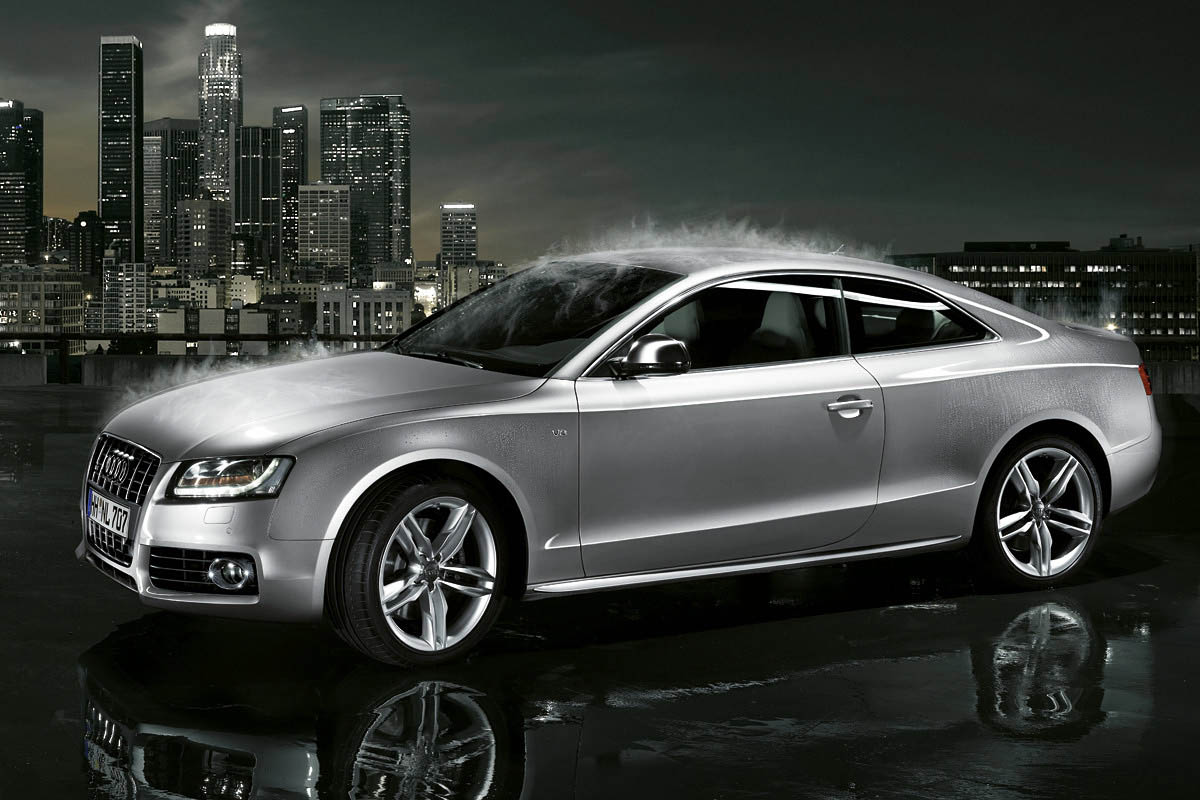
\includegraphics[width=\linewidth]{img/Audi_A5.jpg}
\caption{Audi A5}
\label{fig:image1}
\end{center}
\end{minipage}
\hfill
\begin{minipage}[c]{.55\linewidth}
La chaîne d'énergie d'une voiture est complexe et intéressante à étudier. Les éléments qui la composent sont les suivants: 
\begin{itemize}
 \item moteur,
 \item boîte de vitesse,
 \item réservoir,
 \item roue,
 \item différentiel,
 \item arbre de transmission.
\end{itemize}
\end{minipage}
\end{figure}

\begin{figure}[htbp]
\begin{minipage}[c]{.45\linewidth}
Les chaînes d'énergie et d'information peuvent être très complexes et difficiles à étudier dans leur ensemble comme le montre la figure \ref{fig:image2}, c'est pourquoi, nous allons pour cet exercice utiliser le schéma simplifié de la figure \ref{fig:image3}.
\end{minipage}
\hfill
\begin{minipage}[c]{.5\linewidth}
\begin{center}
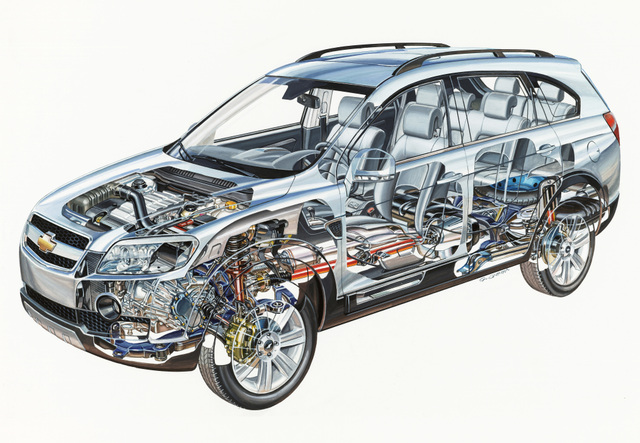
\includegraphics[width=\linewidth]{img/photo_41.jpg}
\caption{Vue ouverte d'une Chevrolet}
\label{fig:image2}
\end{center}
\end{minipage}
\end{figure}

\paragraph{Question 1:}

A la vue du schéma de la figure \ref{fig:image3} et des éléments qui composent la chaîne d'énergie, quelle est l'énergie utilisée pour cette automobile ?

\paragraph{Question 2:}

Compléter la figure \ref{fig:image3} en indiquant, dans chaque case, à quel composant parmi ceux cités plus haut cela correspond.

\begin{figure}[htbp]
\begin{center}
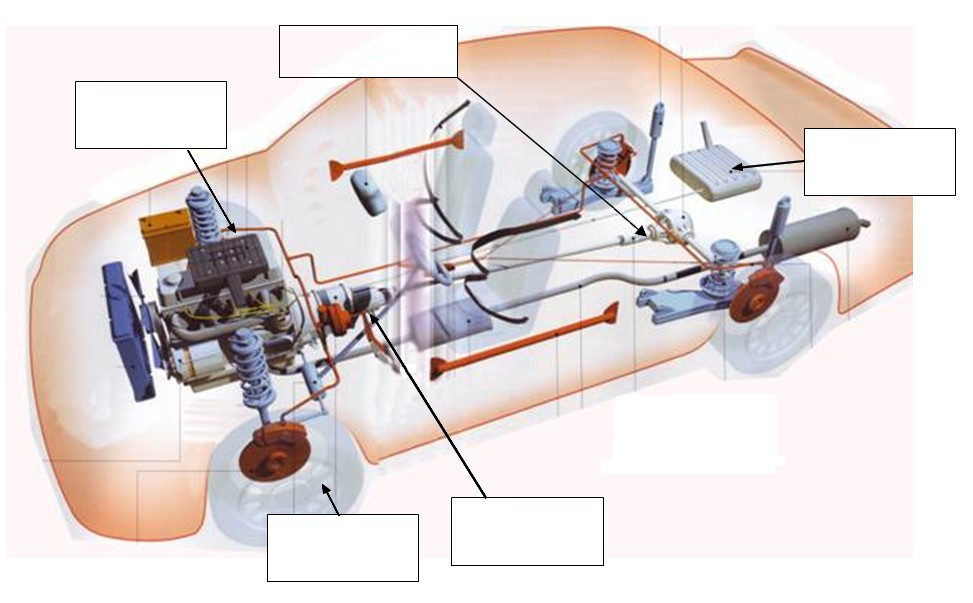
\includegraphics[width=0.8\linewidth]{img/Transmission.jpg}
\caption{Schéma simplifié de la chaîne d'énergie d'une voiture}
\label{fig:image3}
\end{center}
\end{figure}

\newpage

\paragraph{Question 3:}

Tracer le diagramme de définition de blocs de la voiture en utilisant les composants cités précédemment.

\paragraph{Question 4:}

Indiquer à quels maillons de la chaîne d'énergie (Alimenter, Distribuer/Moduler, Convertir, Transmettre, Agir) appartiennent les composants cités.


La combustion dans le moteur de l'énergie d'entrée de l'automobile génère une augmentation de la \textbf{pression} dans la chambre du piston. Cette pression exerce un \textbf{effort} sur le piston, ce qui entraîne un déplacement de celui-ci. La vitesse du déplacement du piston, ainsi que l'effort qui lui est soumis permettent de donner à la voiture de la \textbf{puissance} afin de la mettre en mouvement.

\paragraph{Question 5:}

Donner les unités SI de ces trois grandeurs (pression, effort et puissance) et donner leur équivalent en unités SI de base.

\newpage

\section{Barrage hydroélectrique}


\subsection{Présentation du produit}

\begin{figure}[htbp]
\begin{minipage}[c]{.50\linewidth}
\begin{center}
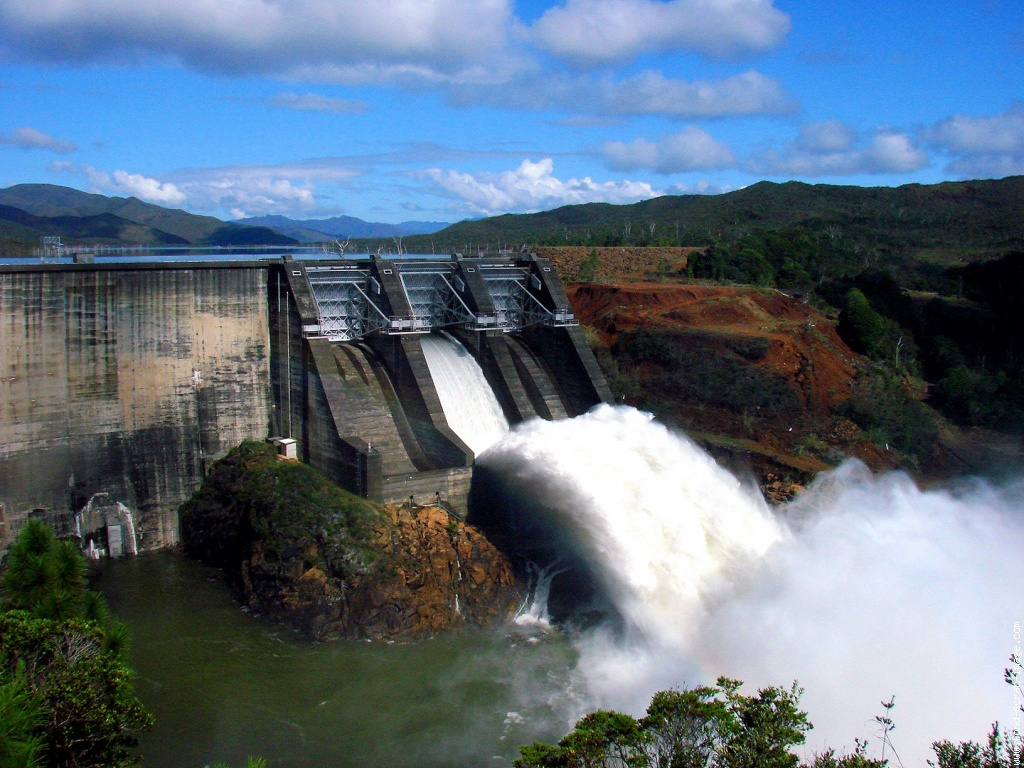
\includegraphics[width=\linewidth]{img/barrage.jpg}
\caption{Barrage}
\label{fig:image4}
\end{center}
\end{minipage}
\hfill
\begin{minipage}[c]{.40\linewidth}
La chaîne d'énergie d'un barrage se compose des éléments suivants: 
\begin{itemize}
 \item alternateur,
 \item lac de retenue,
 \item transformateur,
 \item conduite forcée,
 \item ligne à haute tension,
 \item canal de fuite,
 \item turbine,
 \item barrage.
\end{itemize}
\end{minipage}
\end{figure}

\begin{figure}[htbp]
\begin{minipage}[c]{.55\linewidth}
Les barrages sont en général situés en altitude ou sur des zones à fort courant et installés sur des rivière à fort débit. Des lignes à haute tension permettent alors d'acheminer l'énergie où elle est nécessaire.
\end{minipage}
\hfill
\begin{minipage}[c]{.4\linewidth}
\begin{center}
 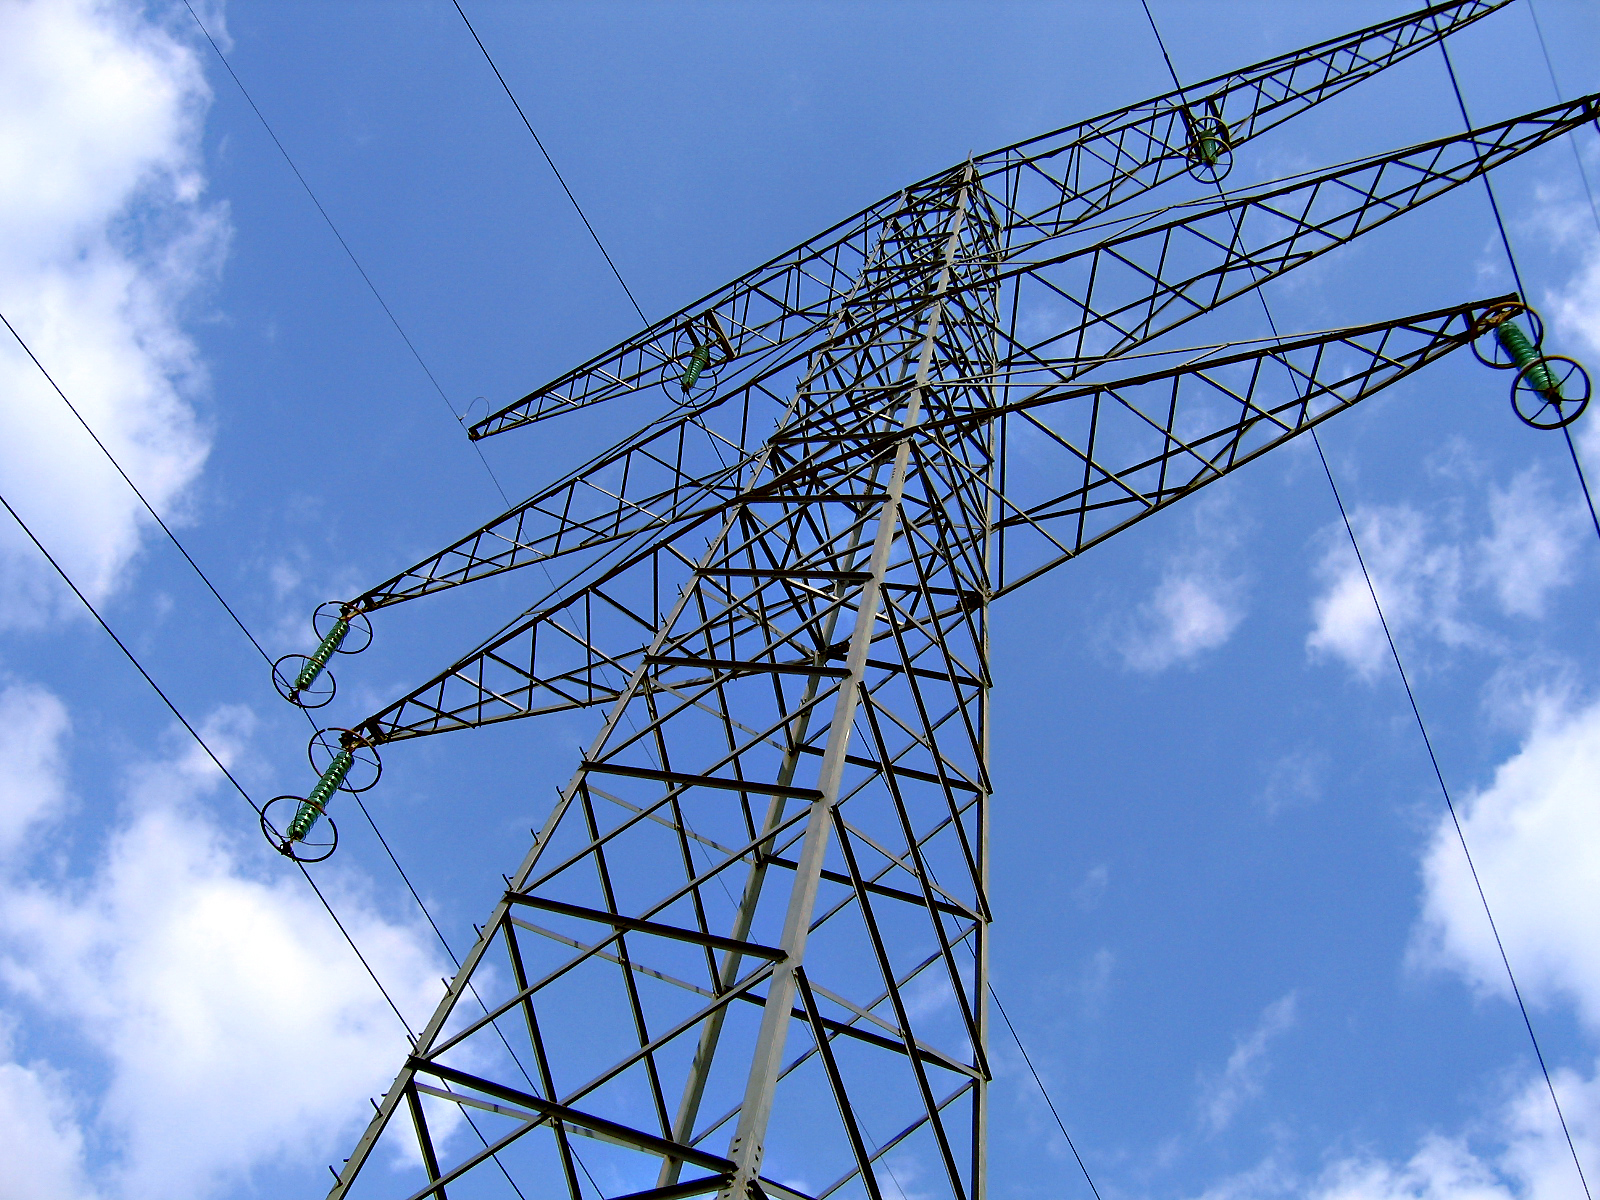
\includegraphics[width=0.9\linewidth]{img/ligne.jpg}
\caption{Ligne électrique}
\label{fig:image5}
\end{center}
\end{minipage}
\end{figure}

\paragraph{Question 1:}

A la vue du schéma de la figure \ref{fig:image6} et des éléments qui composent la chaîne d'énergie, quelle est l'énergie utilisée par le barrage ? Pourquoi le texte à côté de la figure \ref{fig:image5} indique ces précisions?

\paragraph{Question 2:}

Compléter la figure \ref{fig:image6} en indiquant, au dessus de chaque flèche, à quel composant parmi ceux cités plus haut cela correspond.

\begin{figure}[htbp]
\begin{center}
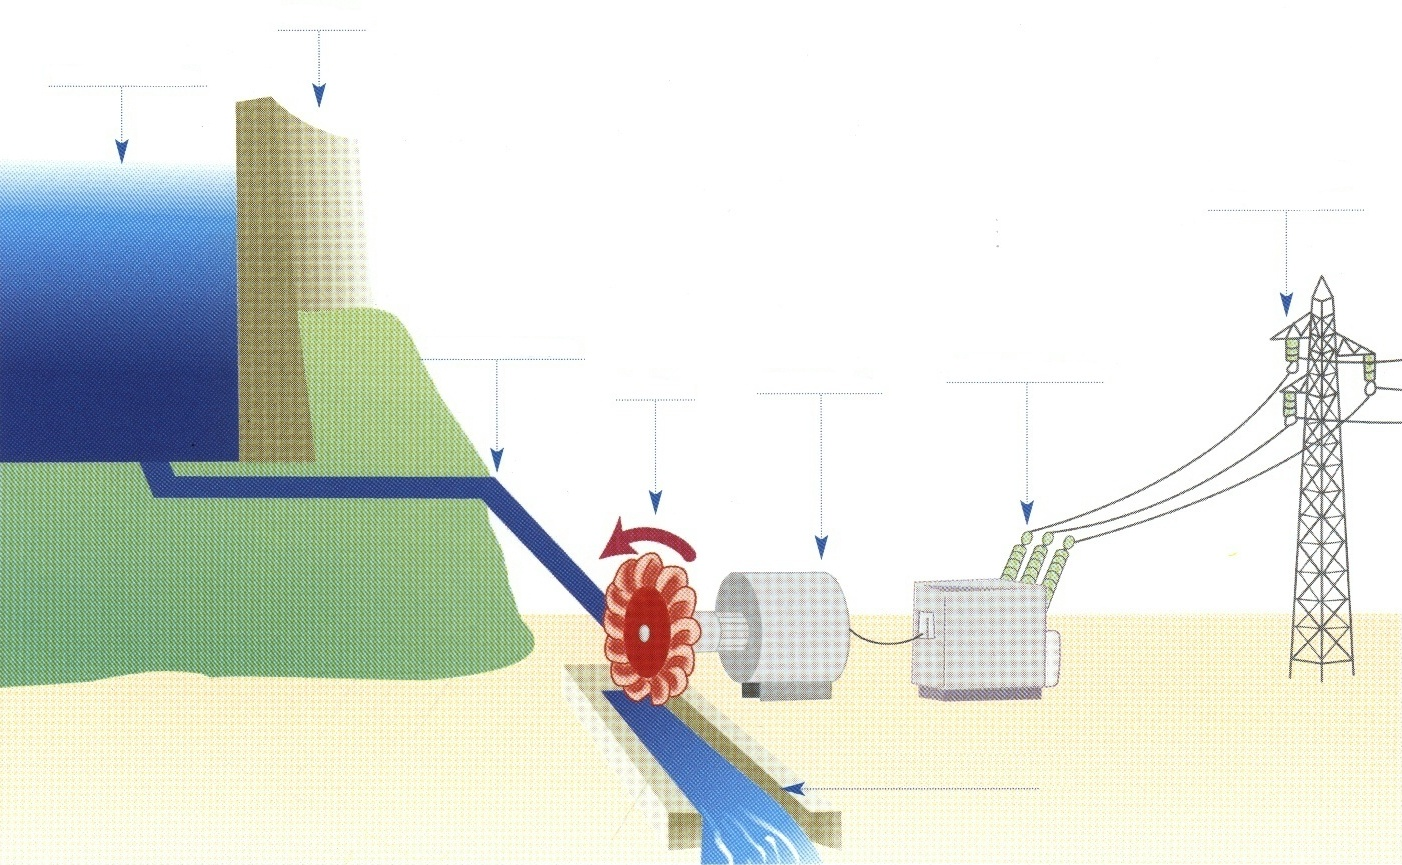
\includegraphics[width=0.9\linewidth]{img/schema_barrage.jpg}
\caption{Schéma simplifié de la chaîne d'énergie d'un barrage}
\label{fig:image6}
\end{center}
\end{figure}


\paragraph{Question 3:}

Tracer le diagramme de définition de blocs du barrage en utilisant un diagramme par composant cité précédemment.

\paragraph{Question 4:}

Indiquer à quels maillons de la chaîne d'énergie (Alimenter, Distribuer/Moduler, Convertir, Transmettre, Agir) appartiennent les composants cités.

Il existe, comme cela est dit plus haut, deux types de barrages (en altitude/sur marée ou sur rivière). Ces deux types de barrage récupèrent l'énergie (en Joule) de l'eau mais dans les deux cas, il ne s'agit pas de la même énergie.

\paragraph{Question 5:}

Donner les types d'énergie utilisés et en utilisant les formules que vous connaissez, montrer que les deux énergies ont le même équivalent en unités SI de base.

\newpage

\section{Chaîne de fabrication de toners}


\subsection{Introduction}

\begin{figure}[htbp]
\begin{minipage}[c]{.35\linewidth}
\begin{center}
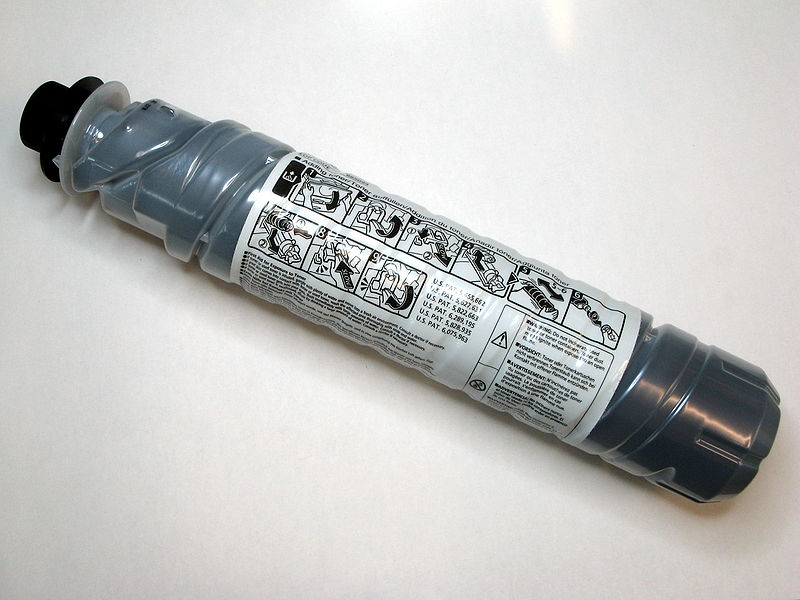
\includegraphics[width=0.9\linewidth]{img/toner.jpg}
\caption{Toner noir}
\label{fig:image8}
\end{center}
\end{minipage}
\hfill
\begin{minipage}[c]{.6\linewidth}
Le toner ou encre en poudre est l'encre utilisée dans les appareils d'impression photo-électrique, procédé appelé « Xérographie » (inventé par la compagnie Xerox), comme les imprimantes laser et les photocopieurs. C'est une poudre, constituée en majeure partie de fines particules de matière plastique, de résine et de pigment magnétique.
\end{minipage}
\end{figure}

\begin{figure}[htbp]
\begin{minipage}[c]{.55\linewidth}
À l'aide d'une charge électrique (statique), l'encre est polarisée pour être transférée sur le papier. Ainsi, l'encre se trouvant dans la cartouche est transportée par un rouleau magnétique sur le cylindre photo-sensible et finalement elle est déposée sur la feuille de papier. L'encre est ensuite fixée de façon permanente sur la feuille en étant chauffée, à environ 180 degrés Celsius, dans l'unité de fusion.
\end{minipage}
\hfill
\begin{minipage}[c]{.40\linewidth}
\begin{center}
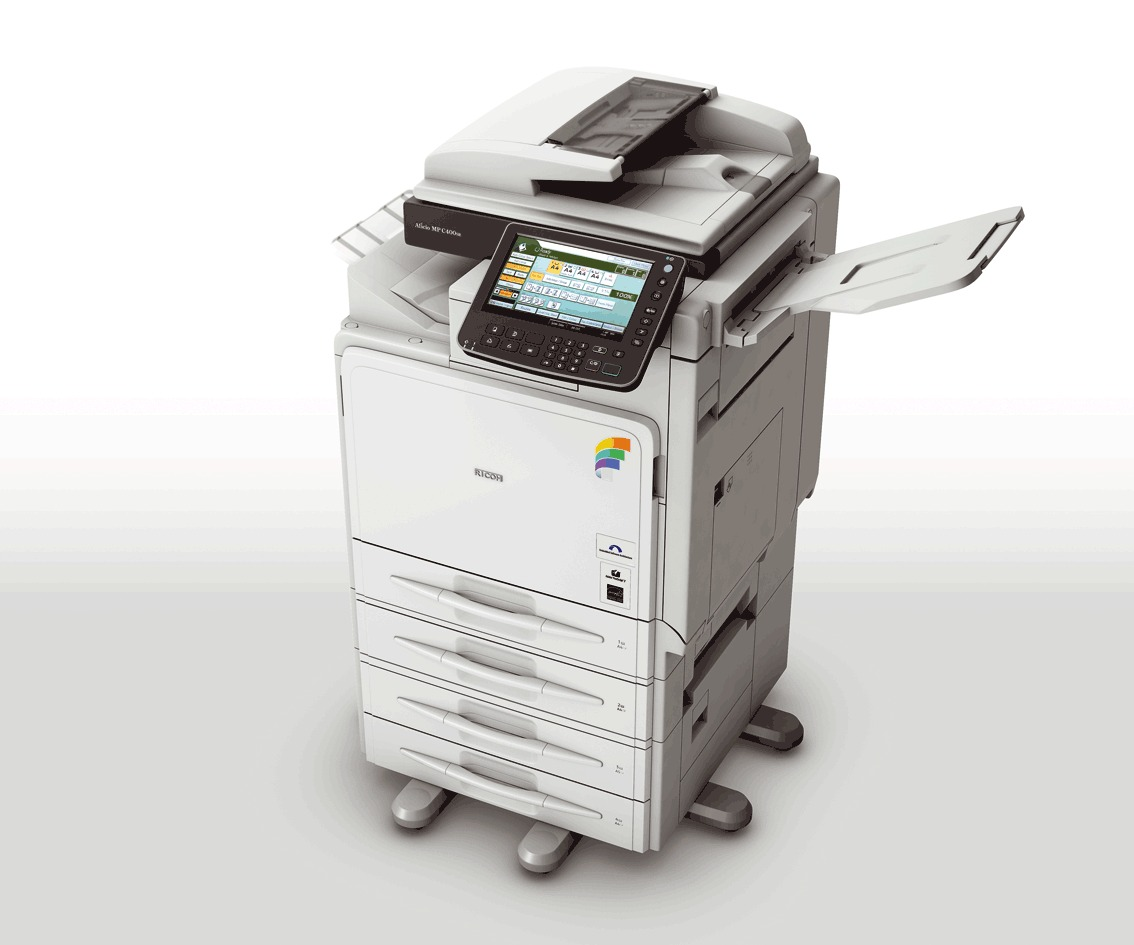
\includegraphics[width=0.9\linewidth]{img/photocopieur.jpg}
\caption{Photocopieur laser}
\label{fig:image9}
\end{center}
\end{minipage}
\end{figure}

\subsection{Présentation du système}

Le schéma de la figure \ref{fig:image7} présente le fonctionnement de la chaîne de production des toners.

\begin{figure}[htbp]
\begin{center}
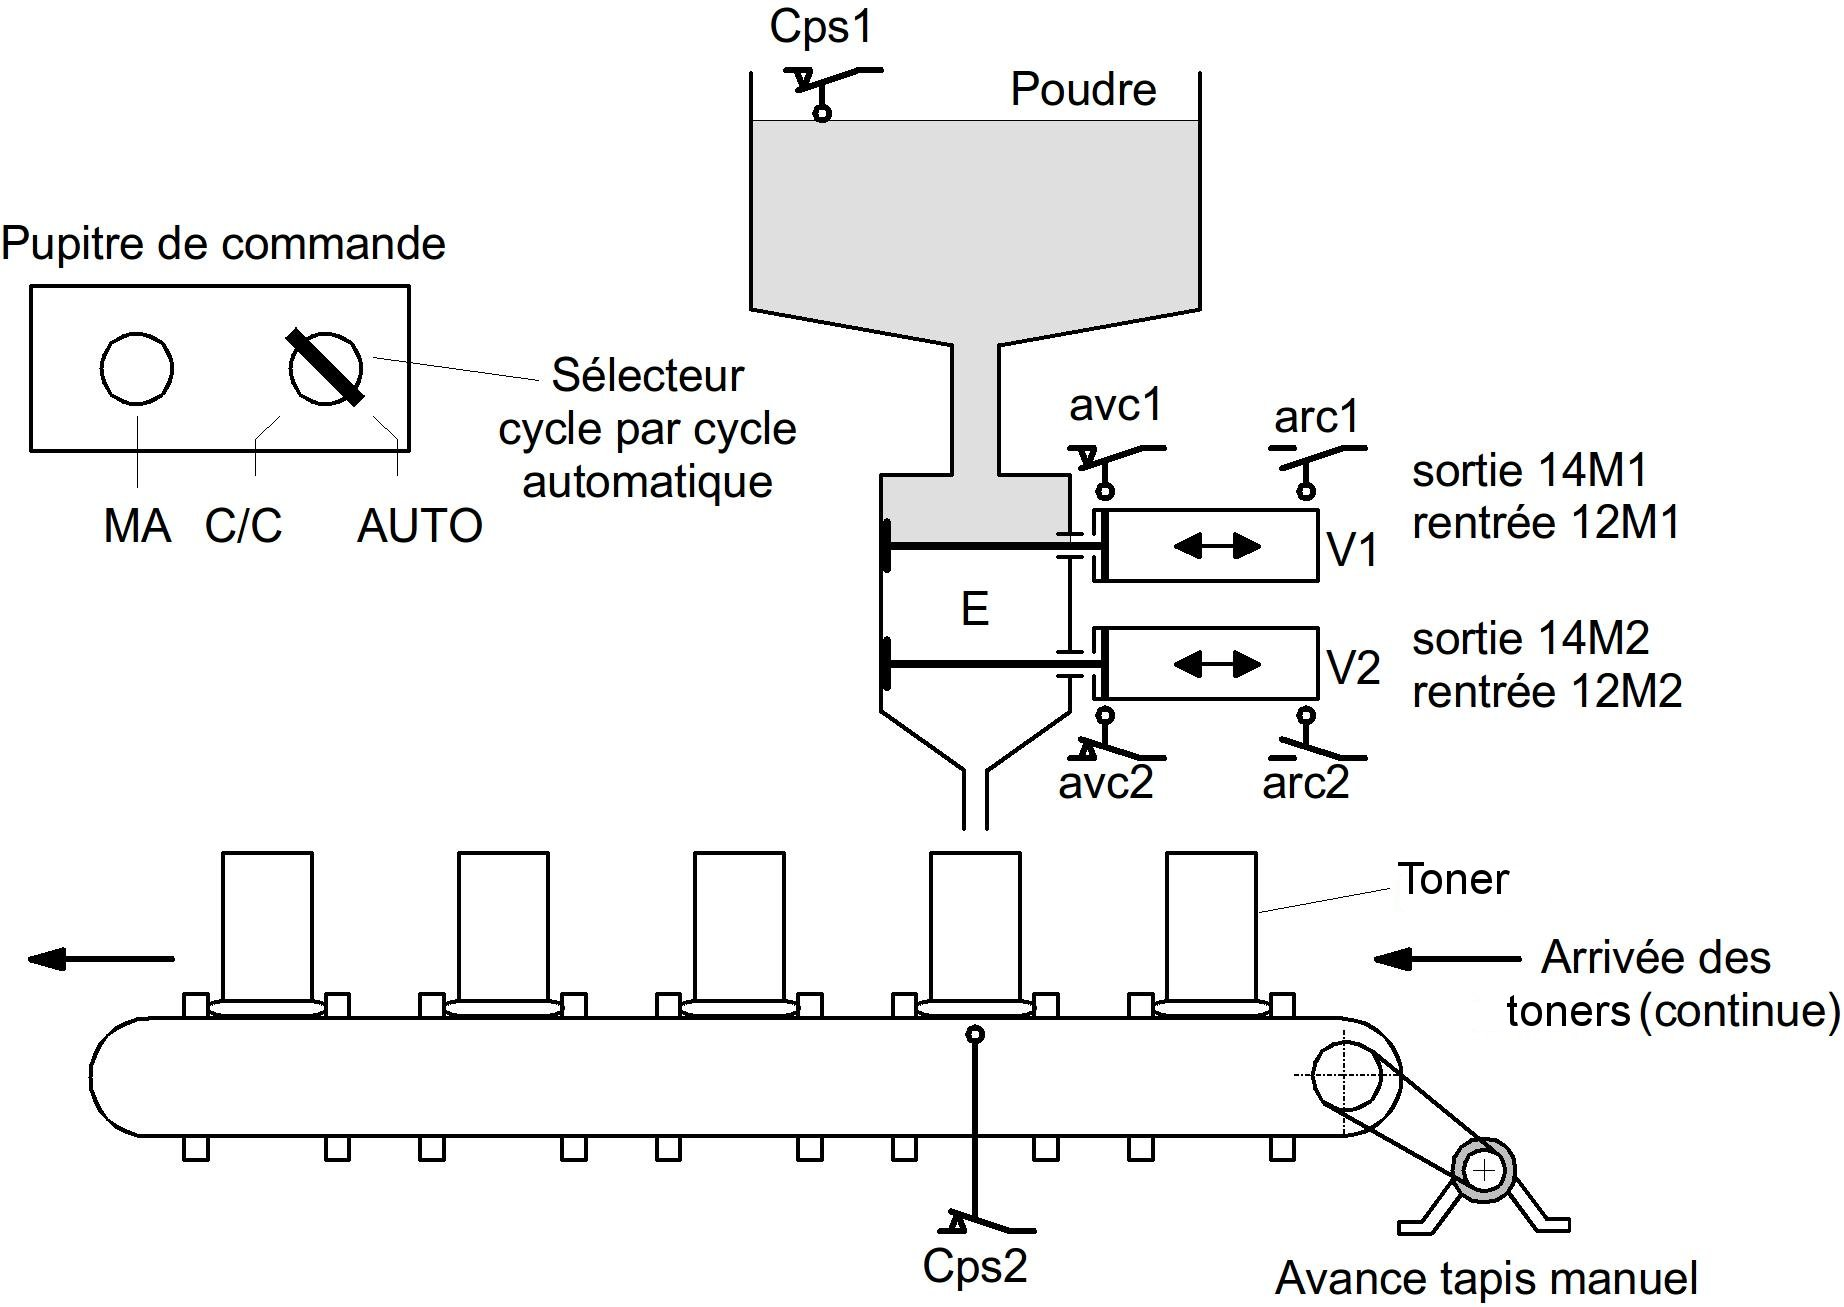
\includegraphics[width=.8\linewidth]{img/ligne_auto.jpg}
\caption{Ligne de production}
\label{fig:image7}
\end{center}
\end{figure}

Ainsi, si les deux vérins V1 et V2 sont sortis et s'il y a présence de poudre dans la trémie de remplissage, un appui sur le bouton poussoir MA fait démarrer le cycle.

Par mouvement successif des vérins V1 et V2, le toner se remplit d'une dose de poudre correspondant au volume E.

En fin de ce cycle 2 cas sont envisageables :
\begin{enumerate}
 \item Le sélecteur est en position automatique et il reste de la poudre dans la trémie, alors le cycle reprend après une intervention de l'opérateur sur l'avance manuel du tapis,
 \item Le sélecteur est en position cycle par cycle et il reste de la poudre dans la trémie, alors le cycle pourra reprendre après une intervention de l'opérateur sur l'avance manuel du tapis  et après appui sur MA par l'opérateur.
\end{enumerate}

\begin{figure}[htbp]
\begin{minipage}[c]{.55\linewidth}
\paragraph{Question 1:}

Tracer le diagramme de blocs interne du système de remplissage des toners.

\paragraph{Question 2:}

Donner pour chaque exemple de capteur utilisé sur le système, un exemple technologique (inductif, optique,...) qui pourrait convenir. Vous pourrez utiliser le tableau \ref{fig:tableau1}.

\paragraph{Question 3:}

Proposer une séquence pour le remplissage d'un toner en utilisant les description des entrées/sorties du tableau \ref{fig:tableau1}. Cette séquence sera écrite sous la forme d'un organigramme qui pourra avoir une forme quelconque.
\end{minipage}
\hfill
\begin{minipage}[c]{.40\linewidth}
\begin{center}
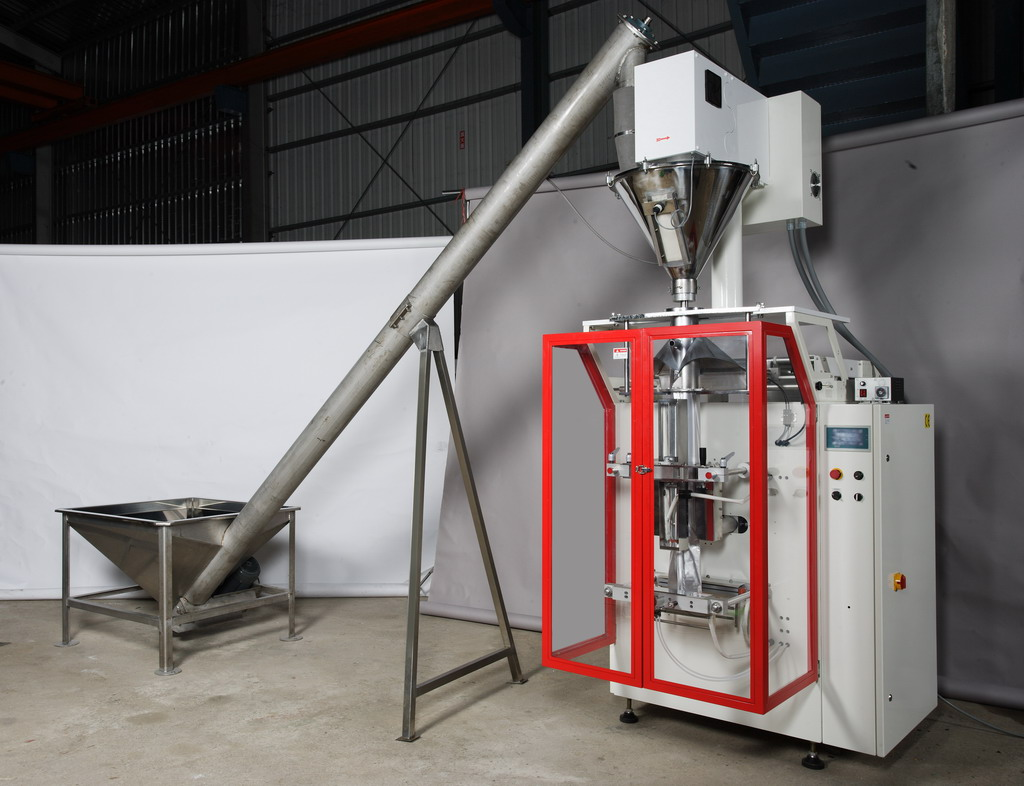
\includegraphics[width=0.9\linewidth]{img/machine.jpg}
\caption{Machine de remplissage}
\label{fig:image10}
\end{center}
\end{minipage}
\end{figure}

\begin{figure}[htbp]
\begin{center}
\begin{tabular}{|c|c||c|c|}
\hline
\multicolumn{2}{|c||}{\textbf{Entrées}} & \multicolumn{2}{c|}{\textbf{Sorties}} \\
\hline
Description & Codage TSX & Description & Codage TSX \\
\hline
Capteur arc1 & Cparc1 & Electrovanne 12M1 & D12m1 \\
Capteur avc1 & Cpavc1 & Electrovanne 14M1 & D14m1 \\
Capteur arc2 & Cparc2 & Electrovanne 12M2 & D12m2 \\
Capteur avc2 & Cpavc2 & Electrovanne 14M2 & D14m2 \\
Capteur S1 & Cps1  & & \\
Capteur S2 & Cps2  & & \\
Bouton poussoir MA & Bps3  & & \\
Com AUTO / CC & Coms8 ou AUTO & & \\
\hline
\end{tabular}
\caption{Tableau des entrées/sorties}
\label{fig:tableau1}
\end{center}
\end{figure}

\newpage

\section{Treuil électrique}


\subsection{Introduction}


\begin{figure}[htbp]
\begin{minipage}[c]{.3\linewidth}
\begin{center}
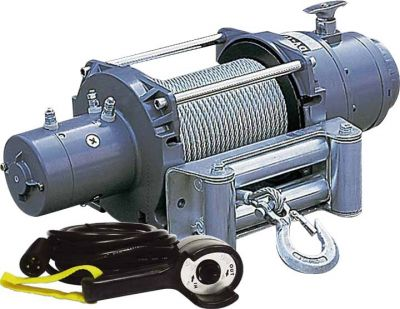
\includegraphics[width=0.9\linewidth]{img/treuil_seul.jpg}
\caption{Treuil}
\label{fig:image11}
\end{center}
\end{minipage}
\hfill
\begin{minipage}[c]{.65\linewidth}
Un treuil est un dispositif mécanique permettant de commander l'enroulement et le déroulement d'un câble, d'une chaîne ou de tout autre type de filin destiné à porter ou à tracter une charge.

Très souvent, il est utilisé afin de soulever de lourdes charges dans des endroits où des personnes sont susceptibles de passer, c'est pourquoi, de nombreuses règles de sécurité sont liées à son fonctionnement.
\end{minipage}
\end{figure}


\subsection{Description du système}

\begin{figure}[htbp]
\begin{minipage}[c]{.55\linewidth}
Le treuil électrique possède les caractéristiques suivantes :
\begin{itemize}
 \item Moteur asynchrone triphasé 220/380 1kW,
 \item Commande par bouton poussoir MO (montée), DE (descente) et STOP,
 \item Bouton poussoir d'arrêt d'urgence,
 \item Alimentation par sectionneur,
 \item Protection moteur par fusible et relais thermique,
 \item Arrêt automatique par capteurs mécaniques de fin de course.
\end{itemize}
\end{minipage}
\hfill
\begin{minipage}[c]{.40\linewidth}
\begin{center}
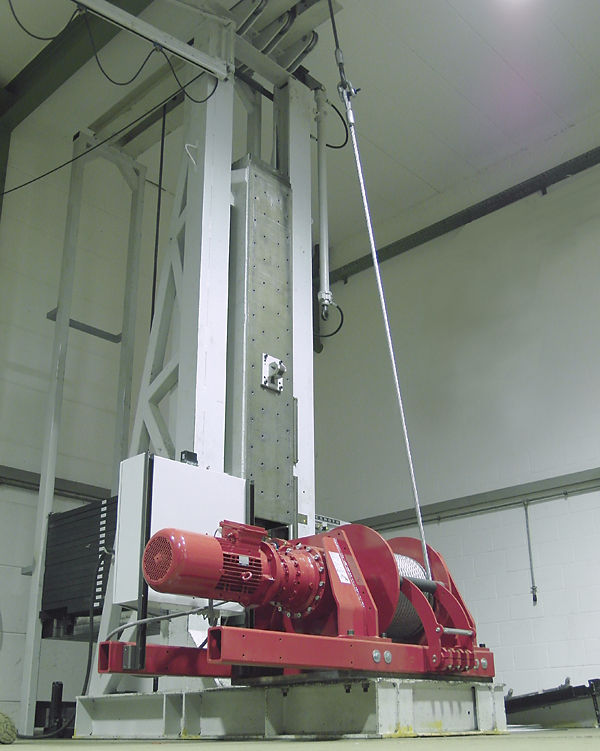
\includegraphics[width=0.9\linewidth]{img/treuil.jpg}
\caption{Câble tendu par un treuil}
\label{fig:image12}
\end{center}
\end{minipage}
\end{figure}

\newpage

\subsection{Étude du schéma électrique}

\begin{figure}[htbp]
\begin{minipage}[c]{.65\linewidth}
\paragraph{Question 1:}

En utilisant les schémas électriques de la partie puissance et de la partie commande présentés ci-après, expliquer le rôle des 4 boutons poussoirs S1, S2, S3 et S4.

~~\\

\paragraph{Question 2:}

Que se passe-t-il s'il on ouvre le sectionneur Q1 lorsque le circuit est en charge. Expliquer l'intérêt du contact de pré-coupure Q1 dans la partie commande.

\end{minipage}
\hfill
\begin{minipage}[c]{.3\linewidth}
\begin{center}
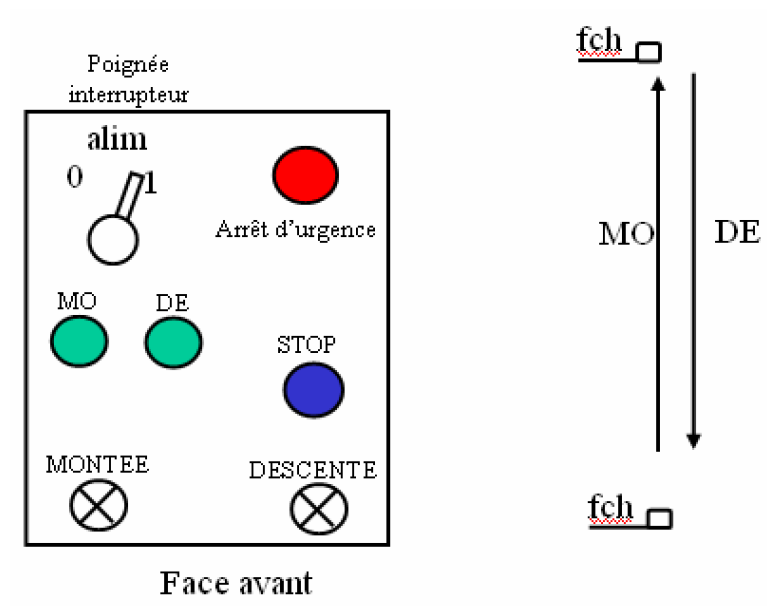
\includegraphics[width=0.9\linewidth]{img/tableau.png}
\caption{Tableau de commande}
\label{fig:image13}
\end{center}
\end{minipage}
\end{figure}


\paragraph{Question 3:}

Donner le but de F1 et le rôle du contact F1 se trouvant dans la partie commande.

\paragraph{Question 4:}

L'utilisateur appuie sur le bouton poussoir S3. Expliquer ce qu'il se passe 

\paragraph{Question 5:}

Expliquer comment KM1 et KM2 permettent la commande du moteur en marche avant et en marche arrière.

\paragraph{Question 6:}

Compléter la partie commande permettant de commander les 2 voyants Montée et descente

\paragraph{Question 7:}

Que se passe-t-il si l'utilisateur appuie simultanément sur les boutons poussoirs S3 et S4 ?

\paragraph{Question 8:}

Un interrupteur différentiel permet de protéger les personnes contre un contact direct. La partie commande ne possède pas d'interrupteur différentiel. Pourquoi ?

\newpage

\begin{figure}[!h]
\begin{center}
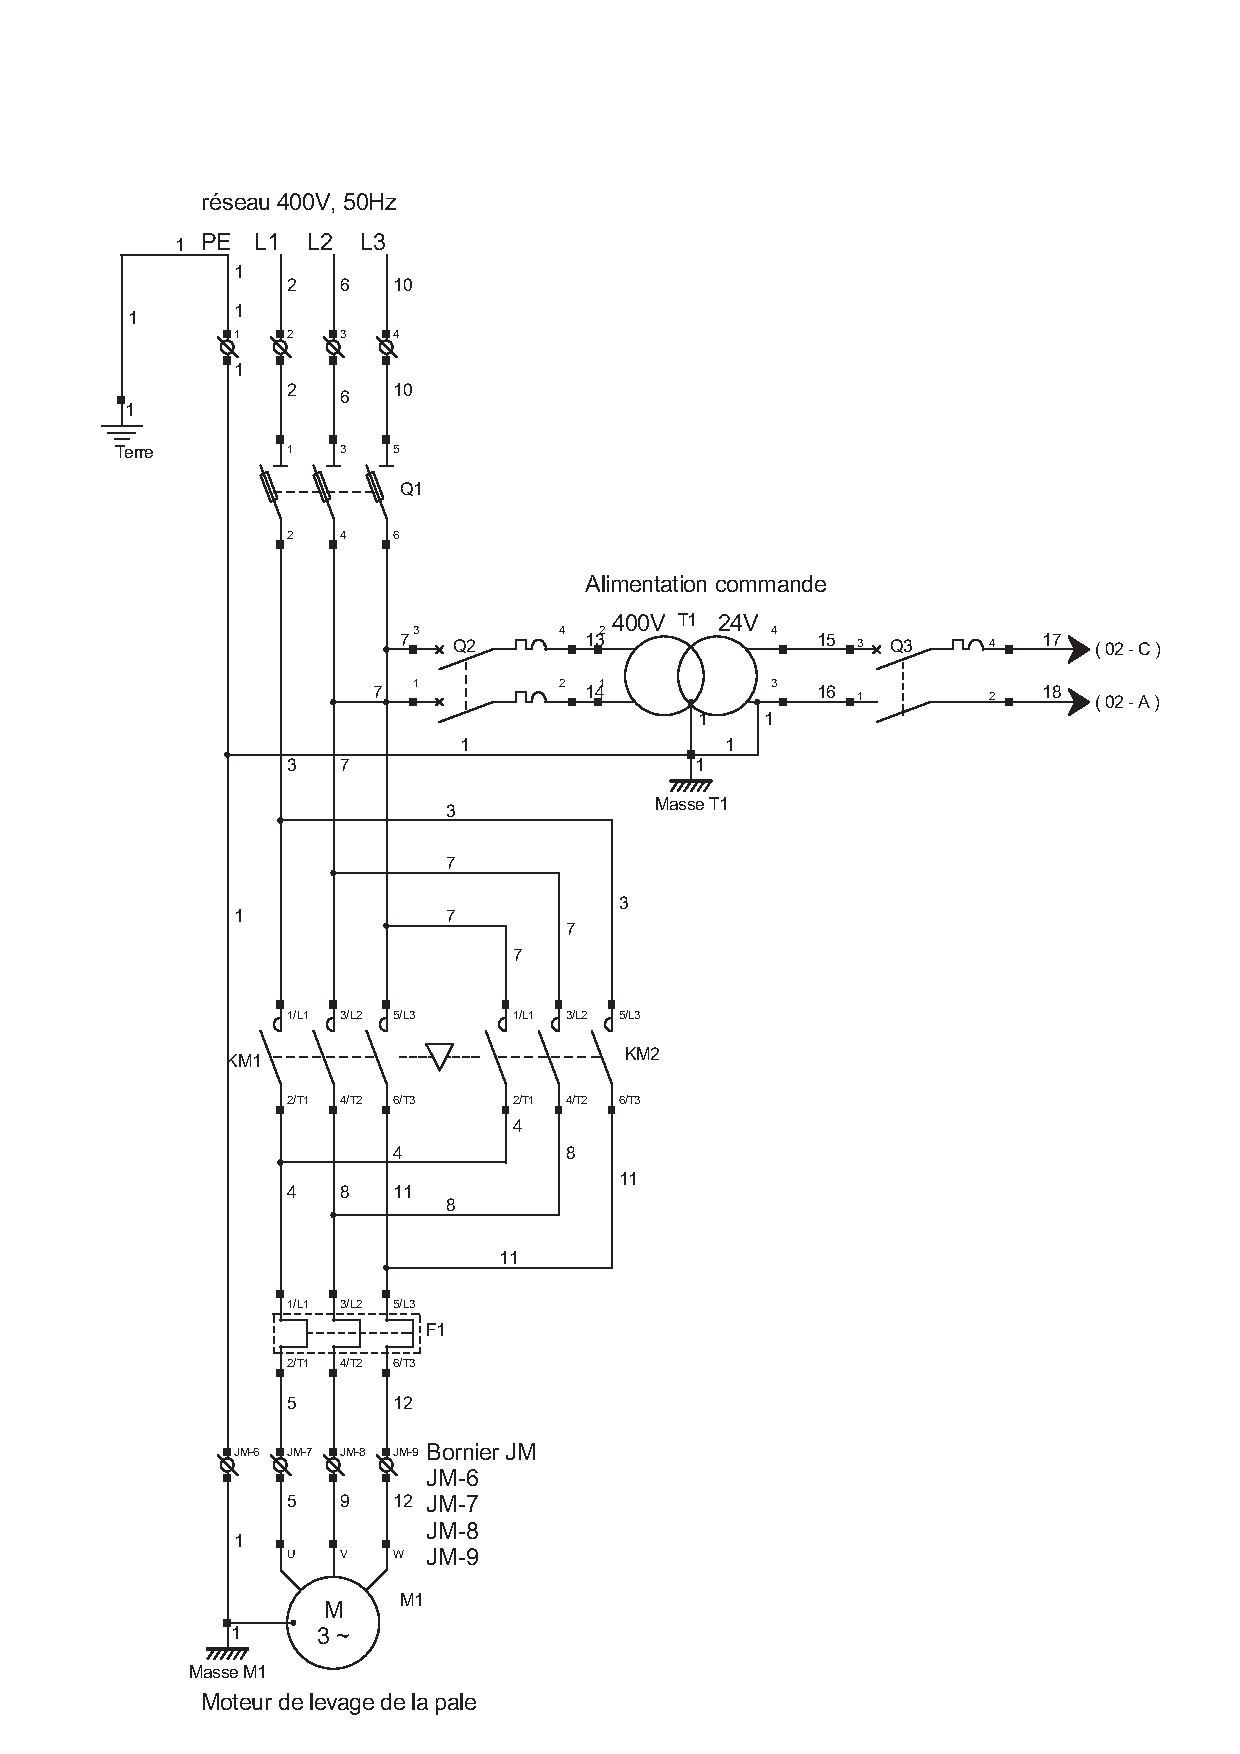
\includegraphics[width=0.9\linewidth]{img/schema1.pdf}
\caption{Schéma électrique de puissance}
\label{fig:image14}
\end{center}
\end{figure}

\newpage

\begin{figure}[!h]
\begin{center}
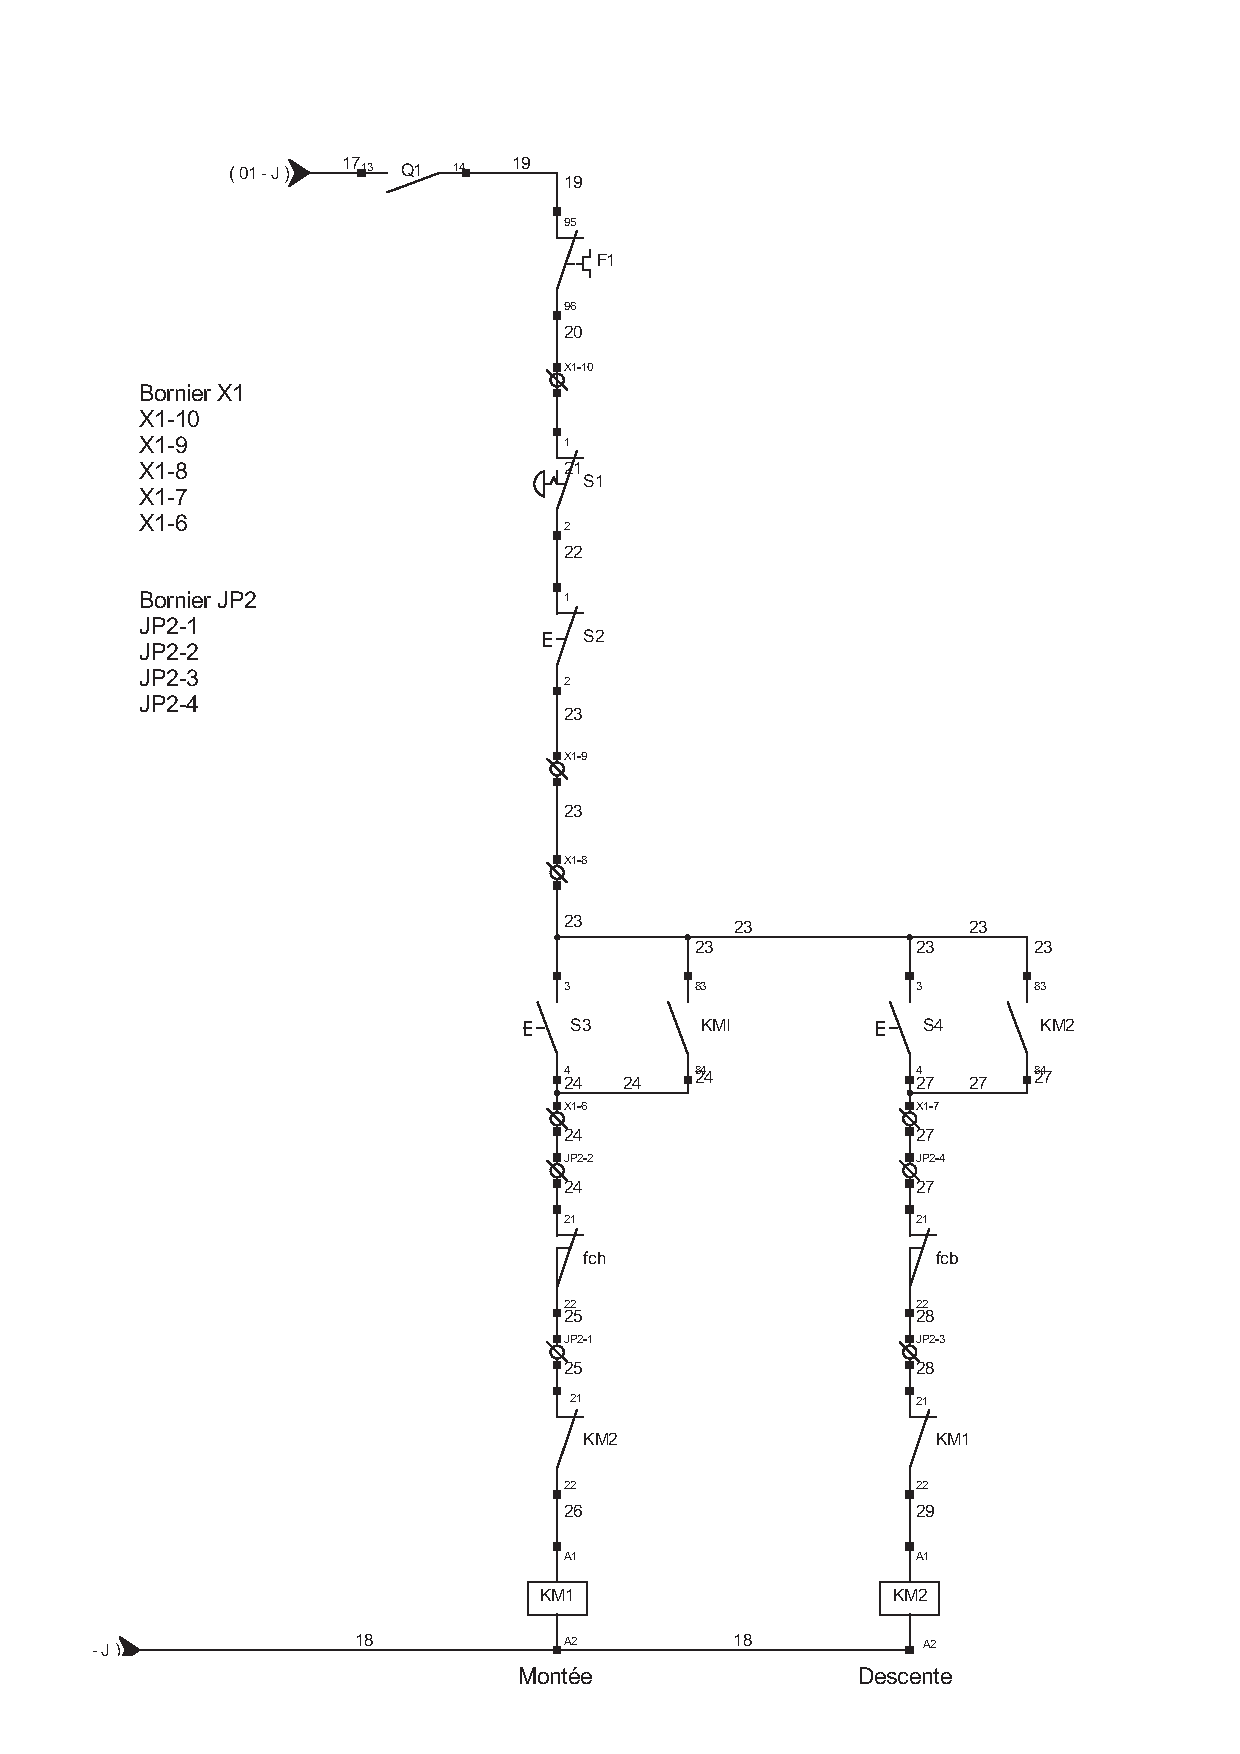
\includegraphics[width=0.9\linewidth]{img/schema2.pdf}
\caption{Schéma électrique de commande}
\label{fig:image15}
\end{center}
\end{figure}


\ifdef{\public}{\end{document}}{}

\newpage

\pagestyle{correction}

\section{Correction}

\subsection{Automobile}

\paragraph{Question 1:} Le stockage est fait dans un réservoir, il s'agit donc d'énergie fossile (essence ou gas-oil).

\paragraph{Question 2:} 

\begin{center}
	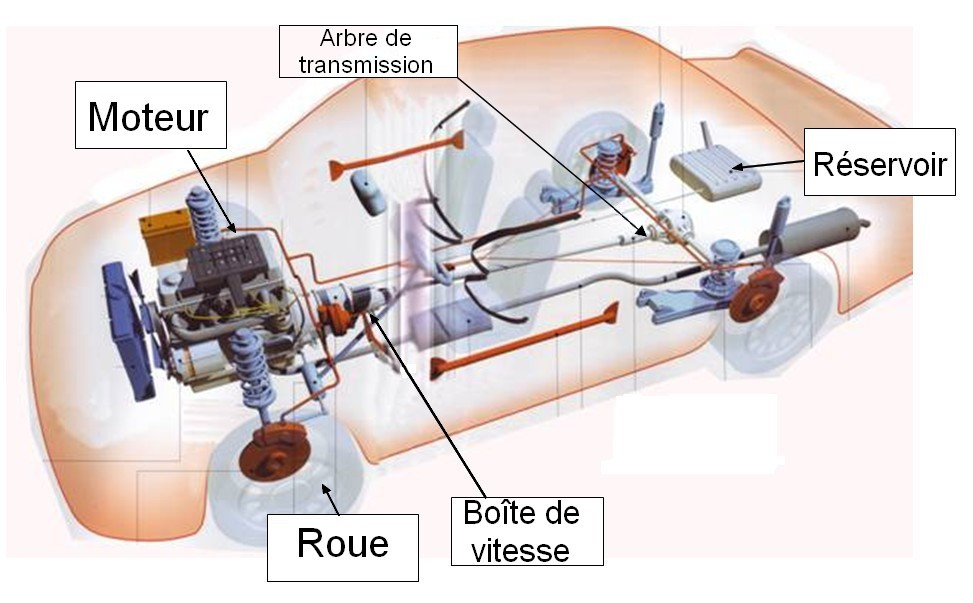
\includegraphics[width=0.6\linewidth]{img/Transmission_cor}
\end{center}

\paragraph{Question 3:}

\begin{center}
	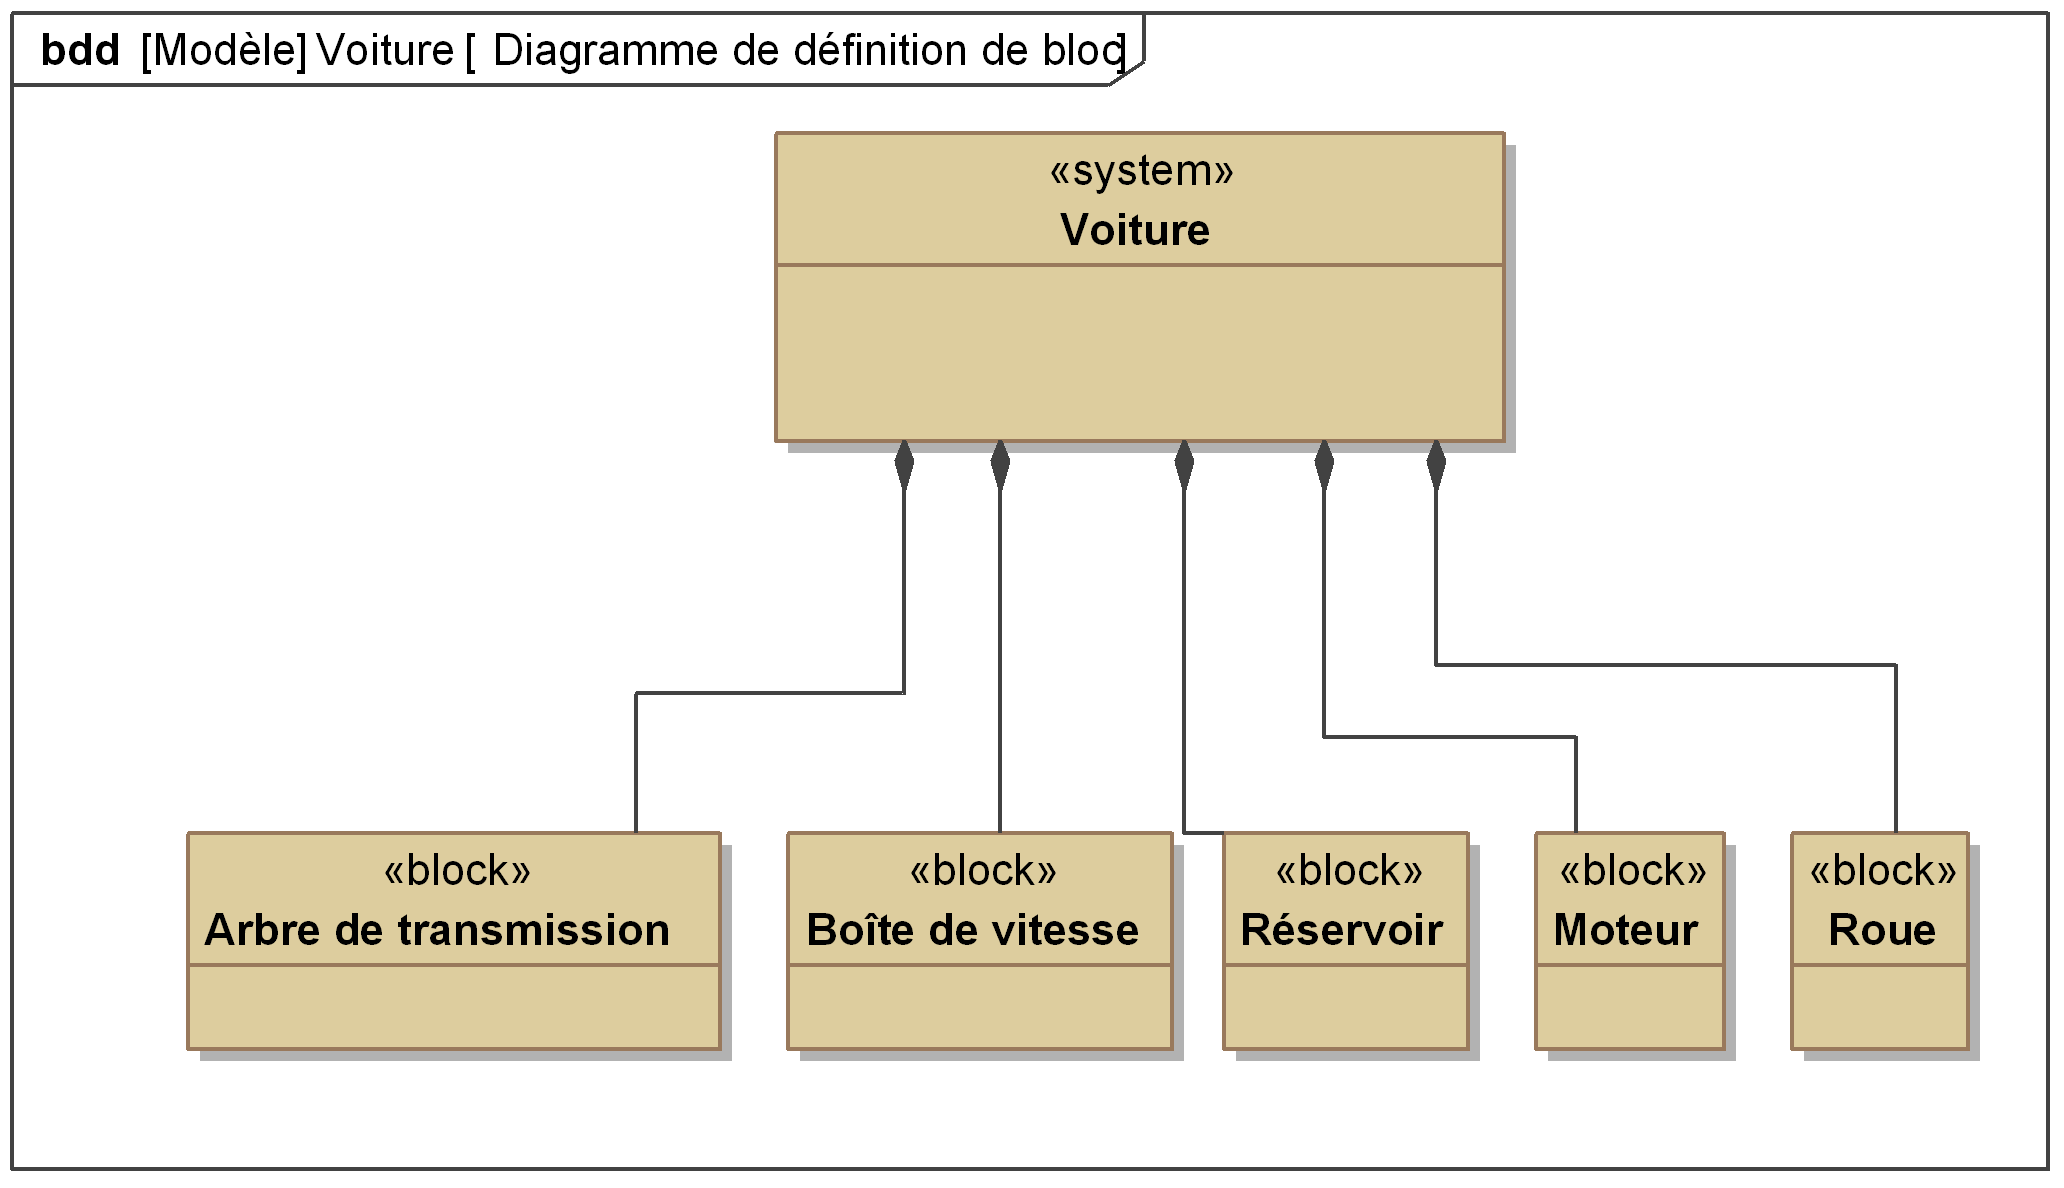
\includegraphics[width=0.6\linewidth]{img/Voiture_bloc}
\end{center}

\paragraph{Question 4:}

Maillons de la chaine d'énergie:
\begin{itemize}
 \item moteur: converti, (distribuer),
 \item boîte de vitesse: transmettre,
 \item réservoir: alimenter,
 \item roue: agir,
 \item différentiel: transmettre,
 \item arbre de transmission: transmettre.
\end{itemize}

\newpage

\paragraph{Question 5:}

\begin{center}
\begin{tabular}{|c|c|c|c|c|}
\hline
Nom de la & Nom de & Symbole & Formule & Unité SI \\
grandeur dérivée & l'unité dérivée & Symbole & mnémonique & Unité SI \\
\hline
Force & Newton & N & $P=m.g$ & $m.kg.s^{-2}$ \\
\hline
Pression & Pascal & Pa & $P=F/S$ & $m^{-1}.kg.s^{-2}$ \\
\hline
Puissance & Watt & W & $P=V.F=C.\Omega$ & $m^2.kg.s^{-3}$ \\
\hline
\end{tabular}
\end{center}

\subsection{Barrage hydroélectrique}

\paragraph{Question 1:} L'énergie utilisée est mécanique, la précision du texte à côté de la figure indique que le fait de mettre le barrage en altitude permet d'obtenir de l'énergie potentielle, et les rivières à fort débit permettent d'obtenir de l'énergie cinétique.

\paragraph{Question 2:}

\begin{center}
	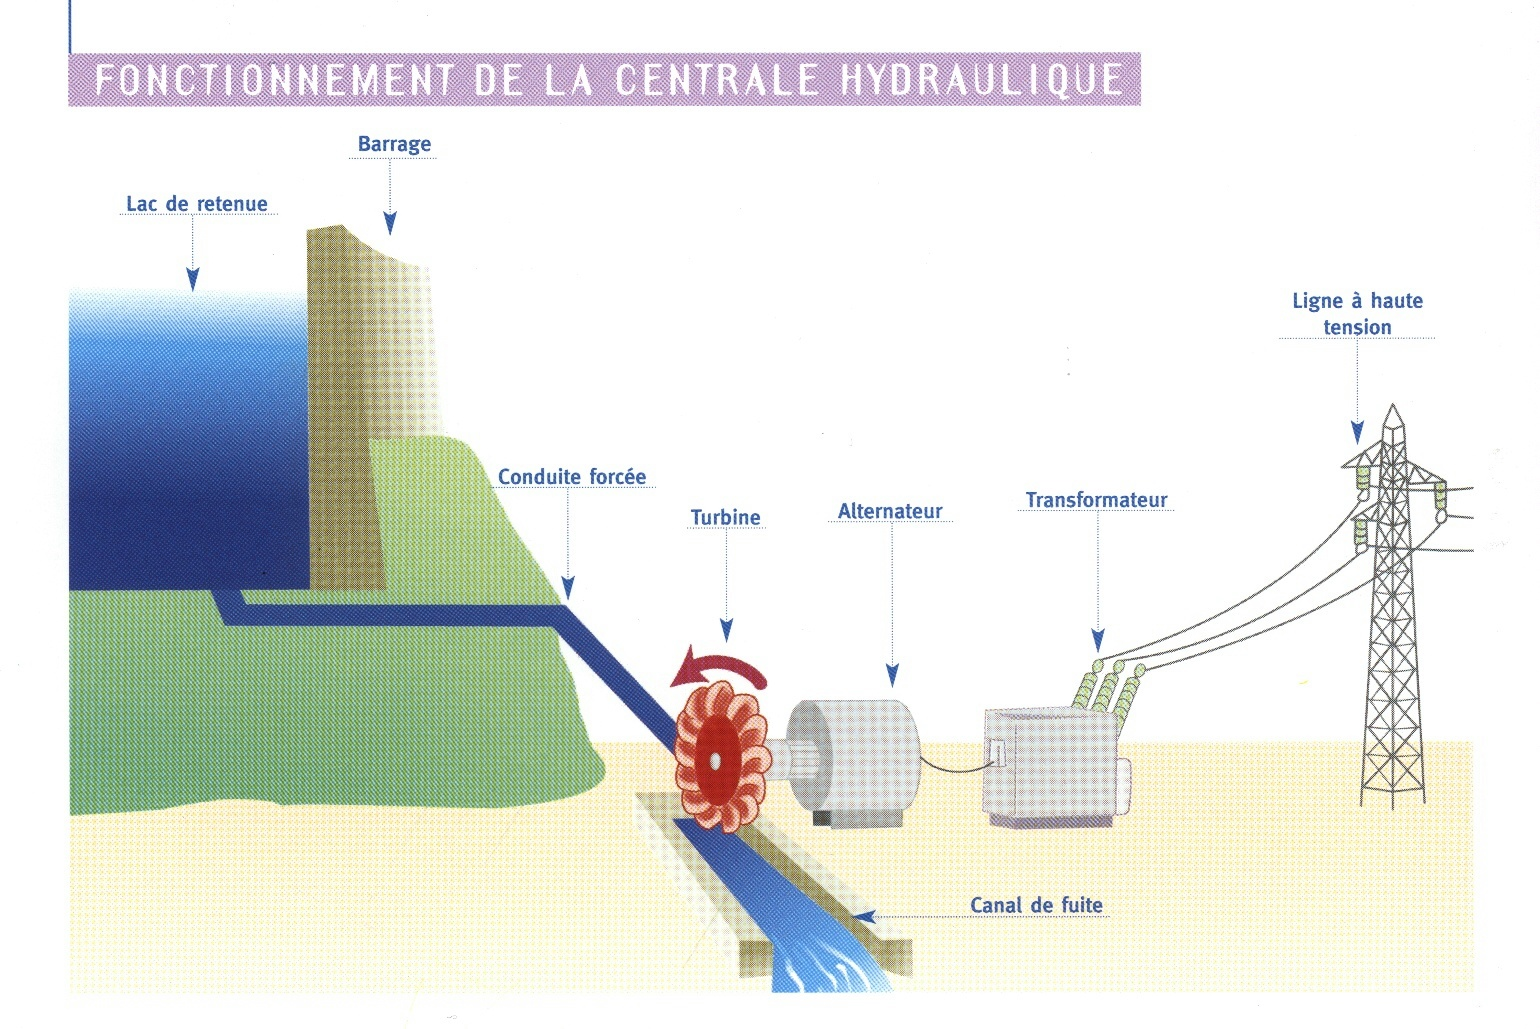
\includegraphics[width=0.7\linewidth]{img/schema_barrage_cor}
\end{center}

\begin{minipage}{0.49\linewidth}

\paragraph{Question 3:}

~\

\end{minipage}
\hfill
\begin{minipage}{0.49\linewidth}

\paragraph{Question 4:}

~\
\end{minipage}

\begin{minipage}{0.49\linewidth}
\begin{center}
	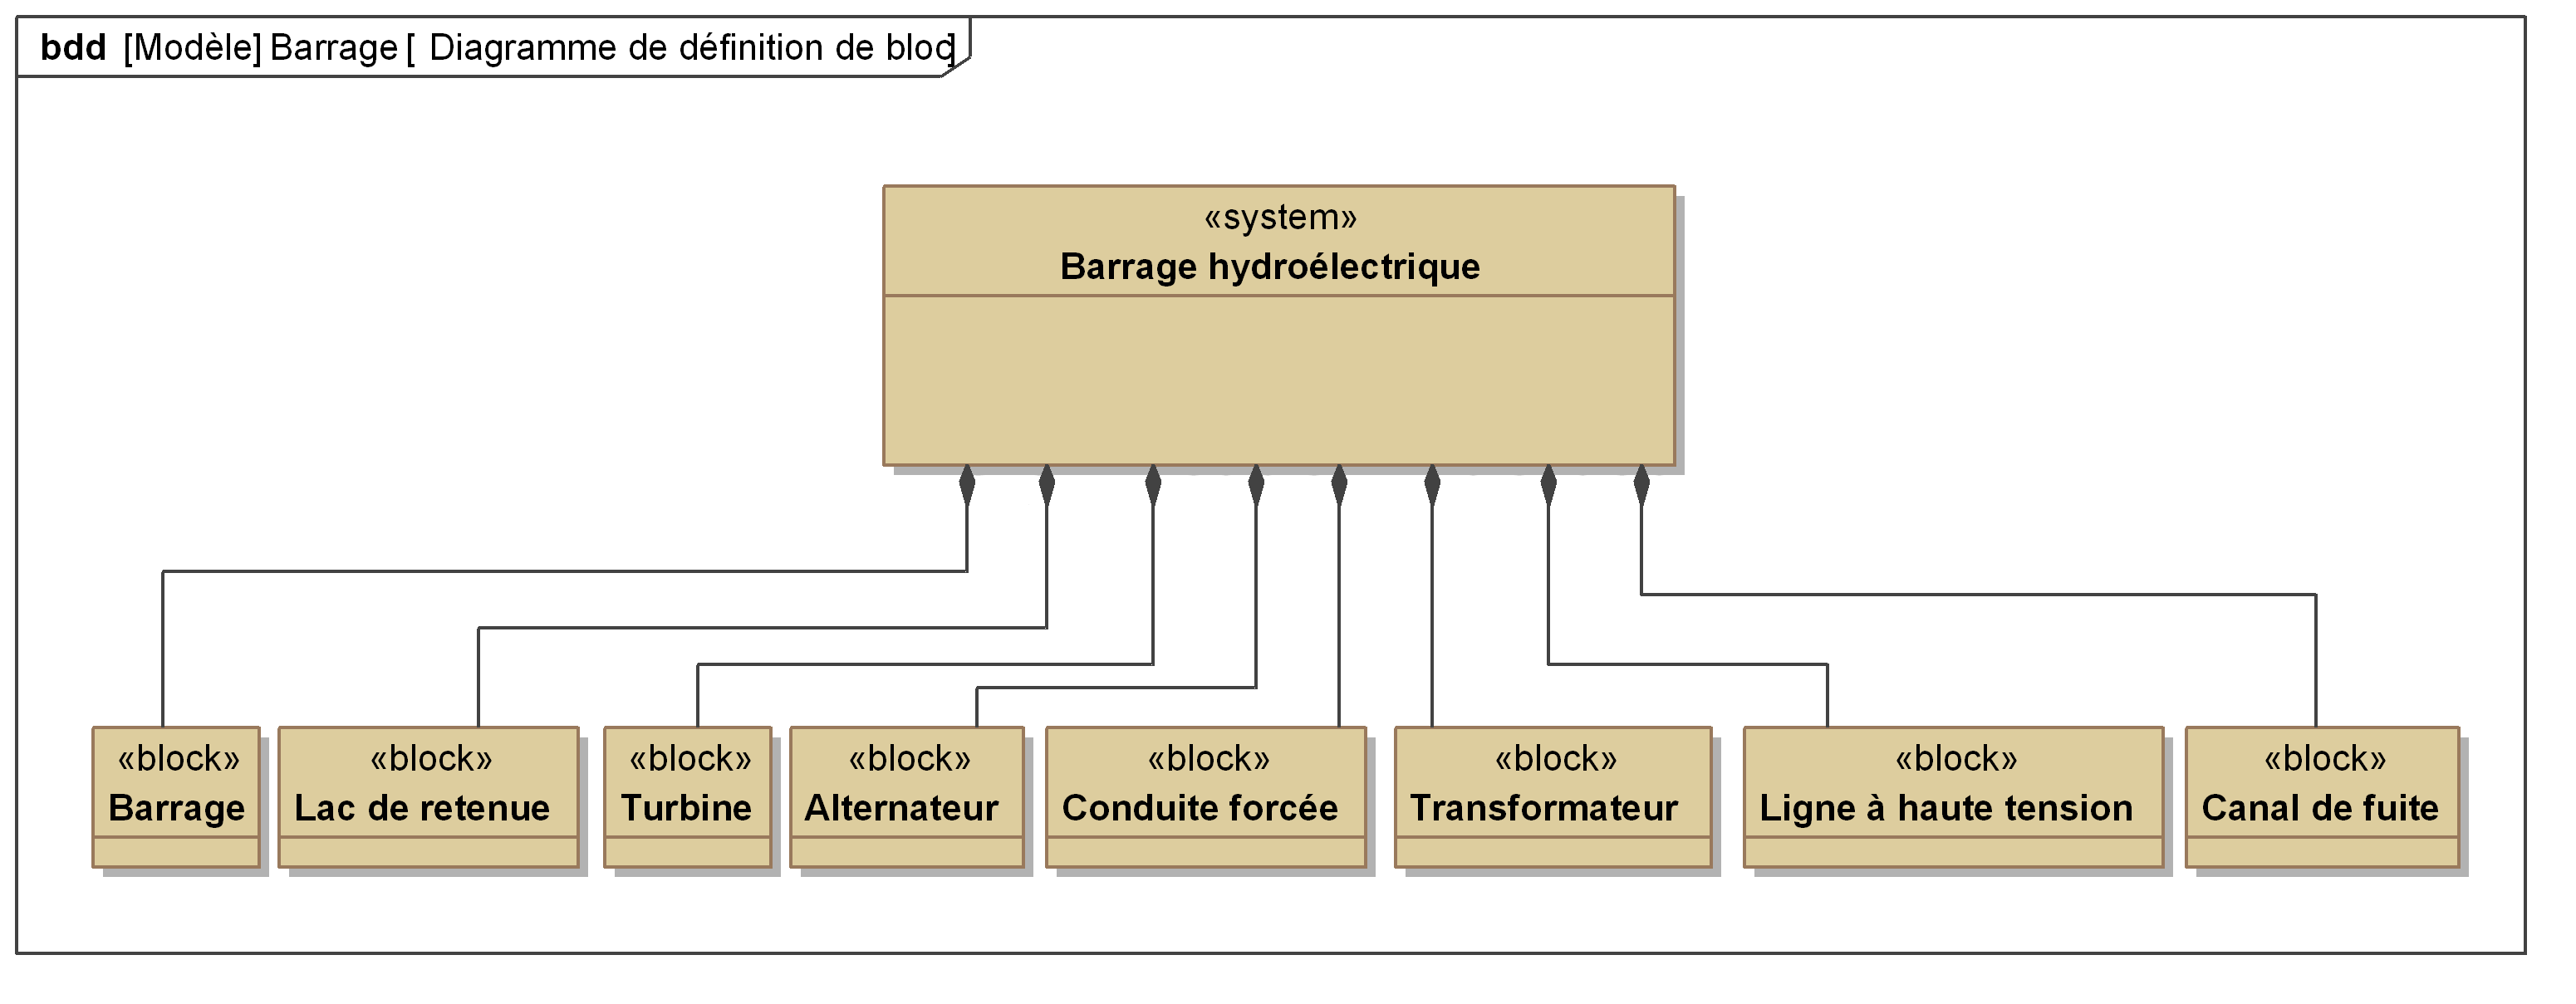
\includegraphics[width=0.9\linewidth]{img/Barrage_bloc}
\end{center}
\end{minipage}
\hfill
\begin{minipage}{0.49\linewidth}
\begin{center}
   \begin{tabular}{|c|c|c|}
	\hline
	Barrage + Lac de retenue & Alimenter \\
	\hline
	Conduite forcée & Distribuer \\
	\hline
	Turbine + alternateur & Convertir \\
	\hline
	Transformateur & Transmettre \\
	\hline
	Ligne à haute tension & Transmettre \\
	\hline
	Canal de fuite & Pertes \\
	\hline
   \end{tabular}
\end{center}
\end{minipage}

\paragraph{Question 5:}

\begin{center}
\begin{tabular}{|c|c|c|c|c|}
\hline
Nom de la & Nom de & Symbole & Formule & Unité SI \\
grandeur dérivée & l'unité dérivée & Symbole & mnémonique & Unité SI \\
\hline
Énergie cinétique & Joule & J & $E=\frac{1}{2}m.v^2$ & $m^2.kg.s^{-2}$ \\
\hline
Énergie potentielle & Joule & J & $E=m.g.h$ & $m^2.kg.s^{-2}$ \\
\hline
\end{tabular}
\end{center}

\newpage

\subsection{Chaîne de fabrication de toners}

\paragraph{Question 1:}

\begin{center}
	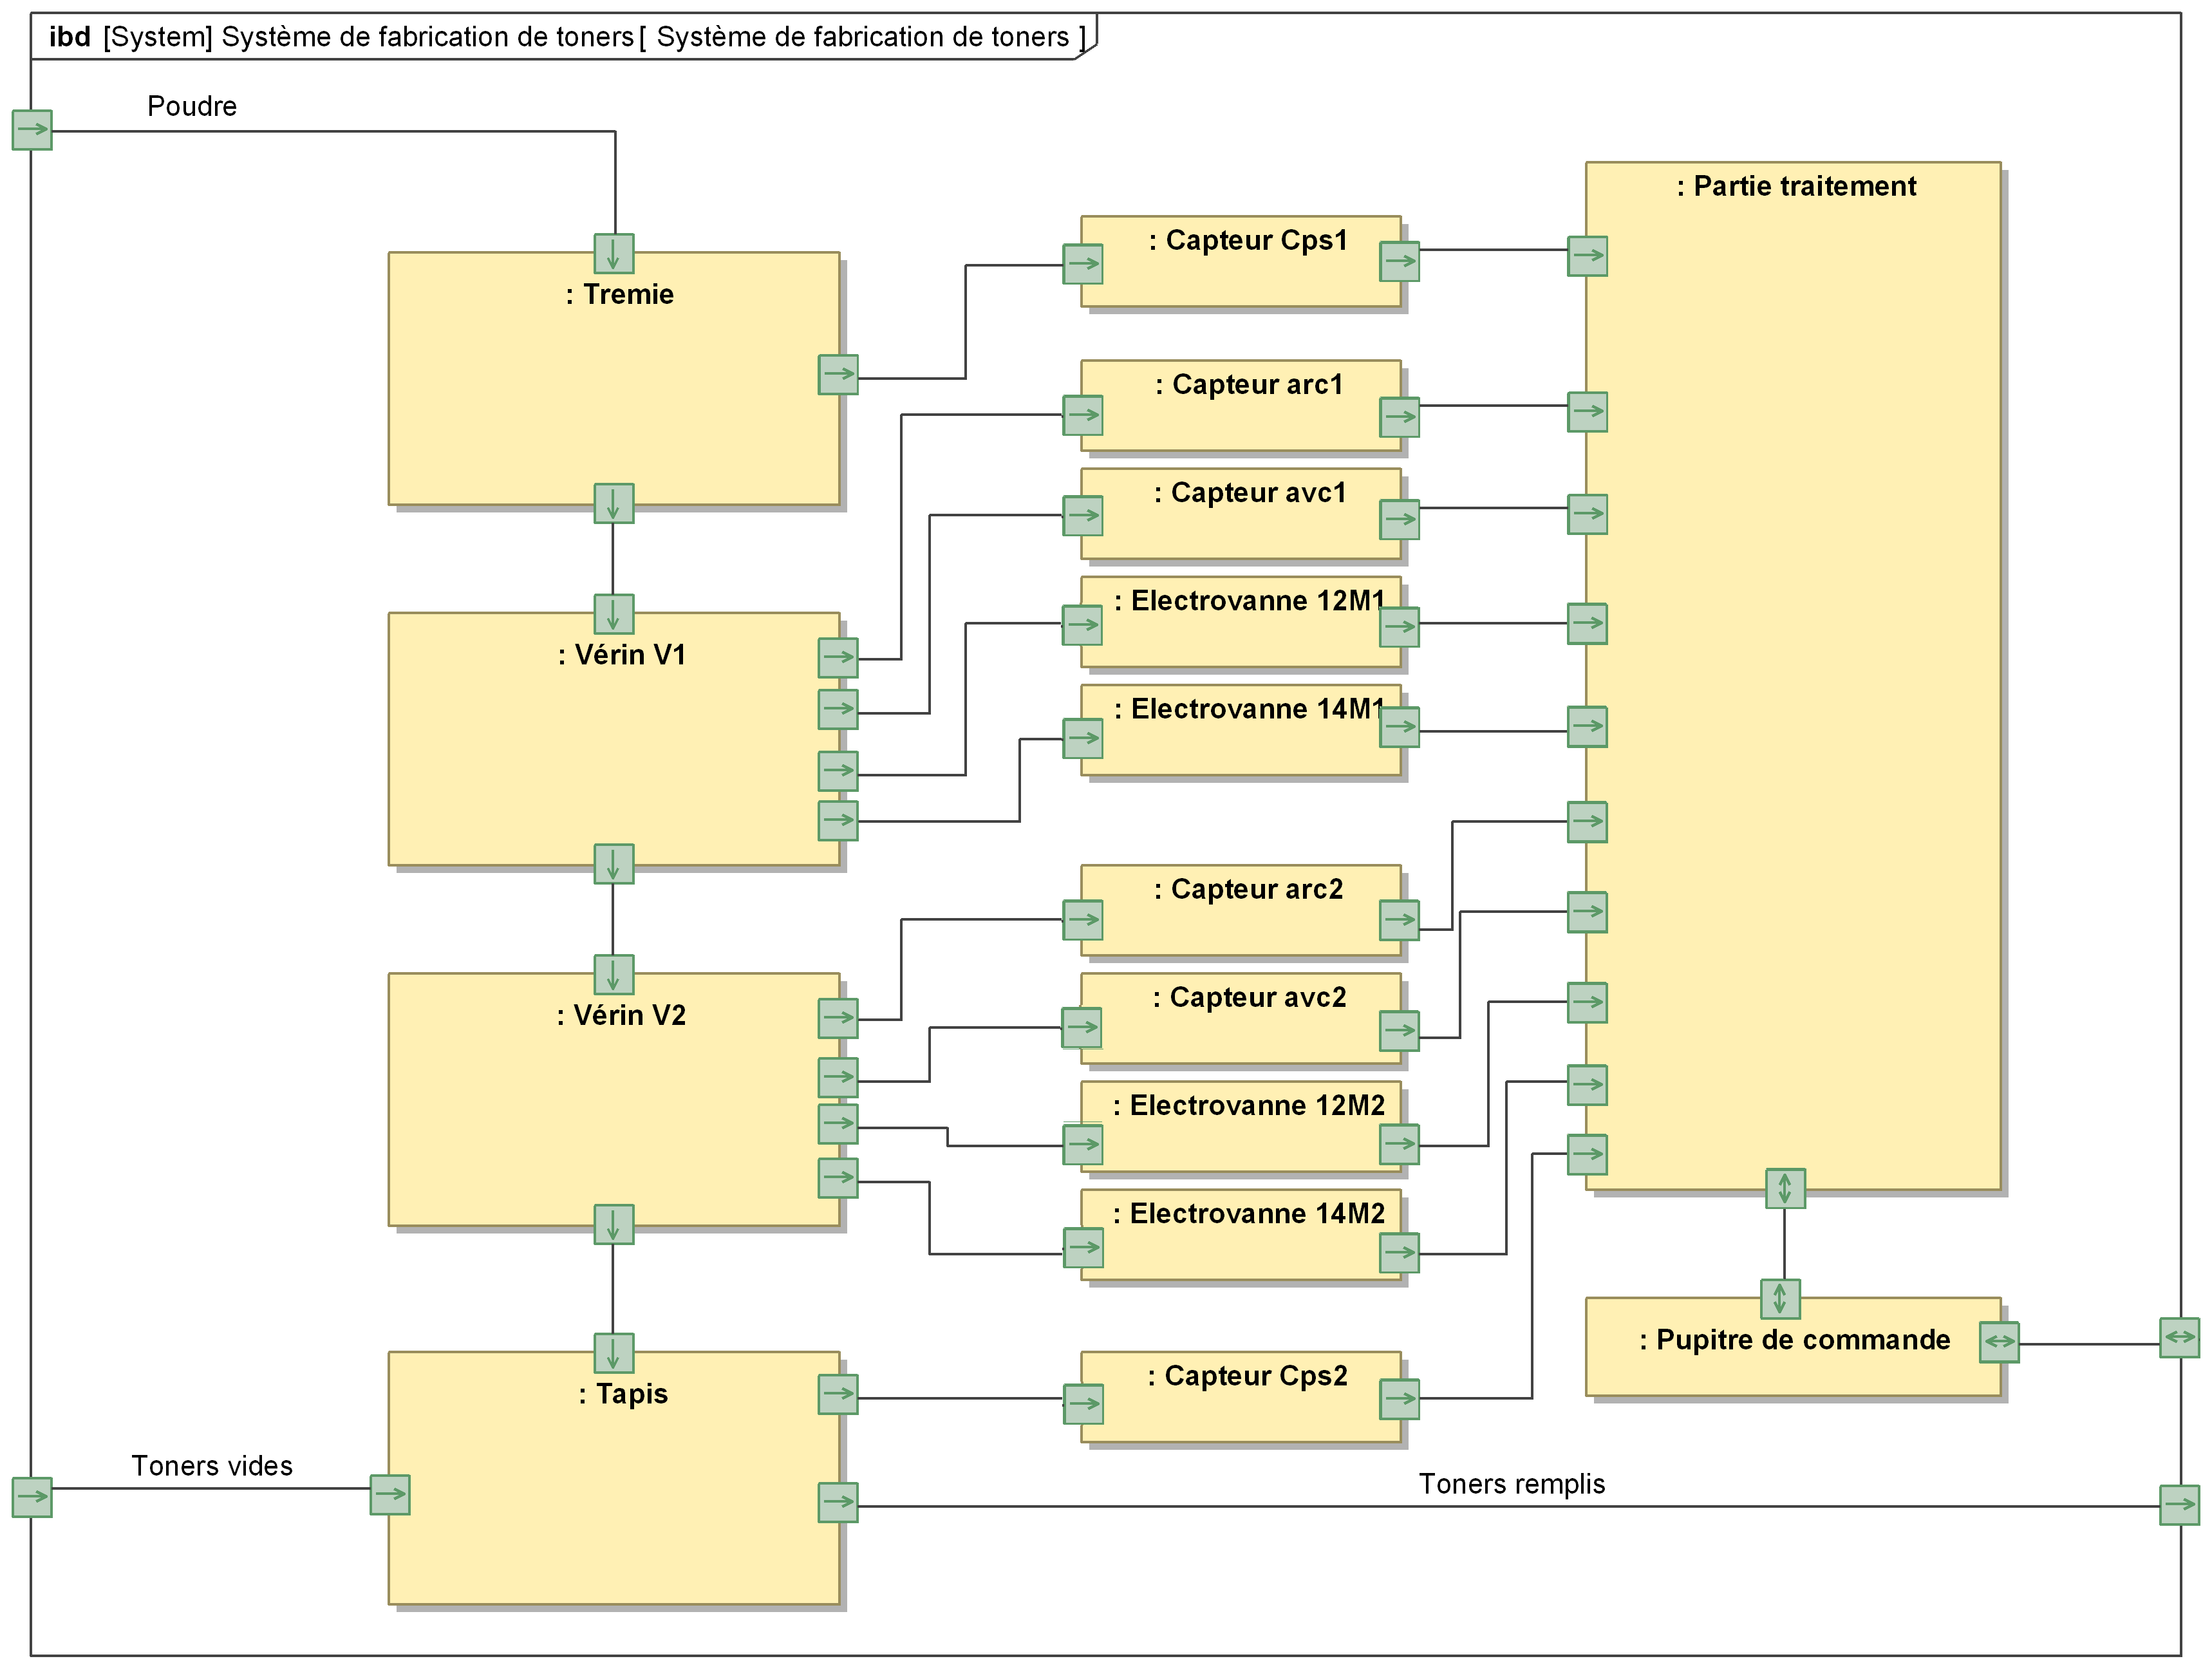
\includegraphics[width=0.8\linewidth]{img/Toners_interne}
\end{center}

\begin{center}
\begin{tabular}{|c|c|}
\hline
Capteur arc1 & Seuil de pression ou ILS \\
\hline
Capteur avc1 & Seuil de pression ou ILS \\
\hline
Capteur arc2 & Seuil de pression ou ILS \\
\hline
Capteur avc2 & Seuil de pression ou ILS \\
\hline
Capteur S1 & Capteur de contact ou optique \\
\hline
Capteur S2 & Capteur de contact, capacitif ou optique \\
\hline
\end{tabular}
\end{center}

\paragraph{Question 2:}

\textit{Conditions initiales: Cps2 détecte l'arrivée d'un toner, Cps1 confirme qu'il y a de la poudre. (Il est possible de considérer que Cps1 sert à détecter l'arrêt du remplissage de la trémie auquel cas il n'a pas à rentrer en compte ici.), avc1=1, avc2=1, arc1=0, arc2=0}

\begin{enumerate}
 \item Rentrée V1 (12M1) \textit{avc1=0, avc2=1, arc1=1, arc2=0}
 \item Sortie V1 (14M1) \textit{avc1=1, avc2=1, arc1=0, arc2=0}
 \item Rentrée V2 (12M2) \textit{avc1=0, avc2=0, arc1=1, arc2=1}
 \item Sortie V2 (14M2) \textit{avc1=1, avc2=1, arc1=0, arc2=0} 
\end{enumerate}

\newpage

\subsection{Treuil électrique}

\paragraph{Question 1:}

\begin{itemize}
 \item S1 est un bouton d'arrêt d'urgence,
 \item S2 est un bouton d'arrêt,
 \item S3 est le bouton de montée,
 \item S4 est le bouton de descente.
\end{itemize}

\paragraph{Question 2:} En coupant Q1 avec un système en charge, on provoque la chute de l'élément porté par le treuil. Il s'agit d'une sécurité visant à empêcher le système de redémarrer au retour de la fermeture de Q1.

Souvent un frein magnétique est là pour éviter ce genre de problème.

\paragraph{Question 3:} F1 est un sectionneur thermique sur la partie opérative. Comme pour Q1, l'interrupteur sur la partie commande permet au système de ne pas redémarrer en cas de réarmement de F1.

\paragraph{Question 4:} Cela provoque la montée du treuil. La mise en place de l'interrupteur lié à la bobine KM1 en parallèle permet l'auto-maintien de l'ordre.

\paragraph{Question 5:} Le passage de KM1 à KM2 a pour effet d'inverser 2 fils d'alimentation du moteur triphasé. Ainsi, cela modifie l'ordre de déphasage des bobines et donc le sens de rotation du moteur.

\paragraph{Question 6:} Les voyants de montée et de descente doivent se situer en série avec les bobines KM1 (montée) et KM2 (descente).

\paragraph{Question 7:} Rien ne va se passer. Par contre en cas de léger décalage, le premier ordre reçu sera validé et empêchera l'autre de s'exécuter.

\paragraph{Question 8:} Cela ne sert à rien car aucune énergie dangereuse ne transite par la partie commande.

\end{document}
